%%%%%%%%%%%%%%%%%%%%%%%%%%%%%%%%%%%%%%%%%%%%%%%%%%%%%%%%%%%%%%%%%%%%%%%%%%%%%%%
%Objetivo: Mapeamento Sistemático da Literatura com o objetivo de avaliar o que
%está sendo proposto de melhorias nas funcionalidades das FGRM
%Autor: Vagner Clementino e Rodolfo Resende
%Criação: Ter Out 11 19:03:45 BRT 2016
%Modificação: qua mar 15 19:34:48 BRT 2017
%Revisão: qua mar 15 22:22:57 BRT 2017
%%%%%%%%%%%%%%%%%%%%%%%%%%%%%%%%%%%%%%%%%%%%%%%%%%%%%%%%%%%%%%%%%%%%%%%%%%%%%%%

\chapter{Mapeamento Sistemático da Literatura}
\label{ch:mapeamento-sistematico}

\section{Introdução}
\label{sec:map-intro}

Os sistemas de software possuem a tendência de evoluir ao longo do tempo e se
adaptar ao seu ambiente de trabalho. As modificações em software são solicitadas
através de uma Requisição de Mudança (RM). Conforme já discutido as RM's são
gerenciadas pelas Ferramenta de Gerenciamento de Requisições de Mudança (FGRM) o
qual possibilita que as diversas partes interessadas, tais como gerentes,
desenvolvedores e clientes coordenem suas atividades e se comunicam entre
si~\cite{bertram2010communication}.

As FGRM's fornecem aos desenvolvedores o gerenciamento de correções de defeitos
e evolução dos artefatos de software. Além disso, também permitem a
implementação de novos recursos, seja no desenvolvimento ou aprimoramento do
software. Um outro benefício importante do uso deste tipo de ferramenta é que as
mudanças podem ser rapidamente identificadas e relatadas aos desenvolvedores.
Além disso, elas também podem ajudar com a estimativa do custo de
desenvolvimento de software, análise de impacto, rastreabilidade, planejamento,
descoberta de conhecimento e compreensão de software~\cite{cavalcanti2013bug}.

No entanto, todos este benefícios não vêm de graça tendo em vista que uma séries
de questões surgem do gerenciamento das RM's conforme discutido com maiores
detalhes na Seção~\ref{ssub:problemas_relacionadas_rm}. Neste sentido, é
importante analisar o estado da arte sobre as melhorias das funcionalidades das
FGRM's para solucionar ou minimizar os problemas relativos à gestão das RM's.

Neste capítulo apresentamos um Mapeamento Sistemático como o objetivo de
identificar os estudos sobre melhorias das funcionalidades fornecidas pelas
FGRM's. A partir de um conjunto de \textit{64} artigos realizamos a
classificação em quatro dimensões de melhoria conforme proposto por Zimmermann e
outros~\cite{zimmermann2009improving} e pelo função desempenhada no processo de
manutenção de software, a partir de um conjunto de papéis discutidas por Polo e
outros~\cite{Polo1999}.

%Naquele estudo o foco foi melhorar as FGRM's visando aumentar a completude do
%que é relatado nas RM's.  Especificamente, o trabalho consistiu em melhorar os
%sistemas de rastreamento de Bugs de quatro maneiras: foco na ferramenta; foco na
%informação; foco no processo; foco no usuário. Os estudos primários também
%foram classificados pelo papel desempenhado no processo de manutenção de
%software, a partir de um conjunto de papéis existentes no processo de manter de
%software~\cite{Polo1999}.

As contribuições desse estudo é uma visão abrangente do estado da arte em sobre
às melhorias das funcionalidades existentes ou a proposição de novas. Através
deste trabalho pesquisadores da área podem encontrar questões abertas e
profissionais da área de desenvolvimento e manutenção de software poderão
encontrar técnicas para o seu trabalho diário que ser utilizadas para melhorar
seus próprios processos e ferramentas.

\todobegin{Necessário revisar a estrutura do Capítulo após revisão}
Este capítulo está organizado conforme descrito a seguir. Na
Seção~\ref{sec:map-metodologia} descrevemos as questões de pesquisa,
apresentamos a metodologia de pesquisa e como os estudos classificados são
explicados.  Na Seção~\ref{sec:mapeamento_resultados} relatamos os resultados do
estudo com relação as dimensões de melhoria e os papéis na manutenção de
software. As ameaças à validade e os trabalhos relacionados são discutidas nas
Seções~\ref{sec:map_limitacoes_ameacas} e~\ref{sec:map_trabalhos_relacionados},
respectivamente.
%Um resumo do capítulo é realizado na Seção~\ref{sec:resumo_capitulo}.
\todoend

\section{Metodologia de Pesquisa}
\label{sec:map-metodologia}

Um \textit{Mapeamento Sistemático da Literatura}, também conhecido como Estudo
de Escopo (Scoping Studies), tem como objetivo fornecer uma visão geral de
determinada área de pesquisa, estabelecer a existência de evidências de estudos
sobre determinado tema e fornecer uma indicação da quantidade de trabalhos na
linha de pesquisa sob
análise~\cite{keele2007guidelines,wohlin2012experimentation}. A pesquisa e a
prática baseadas em evidências foram desenvolvidas inicialmente na Medicina. No
caso da Engenharia de Software o objetivo deste tipo de trabalho é fornecer os
meios pelos quais as melhores evidências atuais da pesquisa podem ser integradas
com a experiência prática e os valores humanos no processo de tomada de decisão
relativo ao desenvolvimento e manutenção de software.

Nesta dissertação empregamos as diretrizes propostas por Petersen e
outros~\cite{Petersen2008} onde definimos um conjunto de questões de pesquisa
que foram utilizadas para guiar a busca e seleção dos estudos primários. Em
seguida, foram construídos esquemas de classificação com base nos dados
extraídos dos artigos. Por fim, foi realizada a análise e sintetização dos dados
com o objetivo de posicionar os estudos em suas respectivas classes da
taxonomia. A estrutura desta seção está de acordo com o processo descrito por
\textit{Petersen e outros}, de modo que cada subseção representa uma das etapas
propostas pelos autores.

\subsection{Questões de Pesquisa}
\label{subsec:map-questoes-de-pesquisa}

O objetivo deste mapeamento sistemático é identificar as novas funcionalidades e
melhorias das existentes propostas na literatura para as FGRM's. Deste modo,
foram definidas as seguintes questões de pesquisa:

\begin{itemize}
	\item \textbf{Questão 01}: \textit{Quais as melhorias e novas
			funcionalidades estão sendo propostas para as FGRM?}
	\item \textbf{Questão 02}: \textit{Quais papéis envolvidos no processo de
			manutenção de software as funcionalidades visam dar suporte?}
\end{itemize}

Na \textit{Questão de Pesquisa 01} estamos interessados em entender como a
literatura sobre as FGRM's está propondo melhorias nas funcionalidades que este
tipo de software oferece ou mesmo por propostas de novas funções. Esta melhorias
tomam por base os diverso problemas relacionados com a gestão das RM's conforme
discutido na Seção~\ref{ssub:problemas_relacionadas_rm}. O objetivo é entender
as técnicas e abordagens adotas nas soluções propostas. Na \textit{Questão de
	Pesquisa 02} o objetivo é descobrir como os diferentes tipos de papéis
existentes no processo de manutenção de software estão recebendo suporte pelos
estudos da área.

\subsection{Pesquisa da Literatura}
\label{subsec:map-pesquisa-literatura}

Para encontrar o conjunto de estudos mais relevantes, bem como eliminar aqueles
que não permitam responder as questões de pesquisas, adotamos os seguintes
critérios para inclusão ou exclusão de artigos no mapeamento:

\begin{itemize}
	\item Critérios de Inclusão
		\begin{itemize}
			\item Artigos
				publicados em conferências e periódicos (journals)
			\item Estudos
				publicados a partir de 2010\footnote{Foram considerados neste
					estudo artigos publicados até maio/2016, data de realização
					da pesquisa nas base de dados.}
			\item Artigos escritos em
				língua inglesa
			\item Artigos disponíveis com texto
				completo
		\end{itemize}
	\item Critérios de Exclusão
		\begin{itemize}
			\item Livros e literatura cinza (gray literature)
			\item Artigos que não possuem relação com FGRM
			\item Estudos duplicados, neste caso foi considerada a versão mais
				completa do trabalho
		\end{itemize}
\end{itemize}

Os estudos primários foram coletados mediante a aplicação de sentenças de buscas
nas seguintes bibliotecas digitais: \textit{IEEE Explore, ACM Digital Library,
	Scopus, e Inspec/Compendex}. No estudo descrito por Dyba e
outros~\cite{dybaa2007applying} verifica-se que o uso de apenas algumas
bibliotecas digitais apresenta um resultado semelhante que uma configuração
quase exaustiva de base de dados. Em resumo, o conjunto selecionado de
bibliotecas digitais no permite alcançar resultados relevantes.

As sentenças de buscas foram produzidas com base na metodologia PICO
(Population, Intervention, Comparison and Outcomes) que é sugerida por
Kitchenham e Charters~\cite{keele2007guidelines} para ajudar pesquisadores na
formulação de termos tomando como ponto de partida as questões de pesquisa. As
sentenças aplicadas a cada base de dados são apresentadas no
Apêndice~\ref{ch:app-instrumentos-mapeamento}.

Após uma busca automatizada nas base de dados chegamos a um total de 286
artigos. A Tabela~\ref{tab:estudos-por-base-dados} exibe o total de estudos
recuperados por base de dados.  Os trabalhos coletados foram avaliados, através
da ferramenta \textit{JabRef}\footnote{\url{https://www.jabref.org/}}, em busca
de possíveis duplicados. Esta etapa resultou na exclusão de 81 documentos, desta
formal chegamos a 205 estudos ao final do processo. Finalmente os artigos foram
analisados com base na leitura do título e resumo. Nos casos em que o título e
resumo não eram capazes de caracterizar o estudo foi realizada uma leitura
completa do texto. O processo descrito resultou em \textbf{64} estudos. A
Figura~\ref{fig:diagrama-processo-selecao} resume o processo de seleção
apresentado o número de artigos em cada etapa.

\begin{figure} \centering 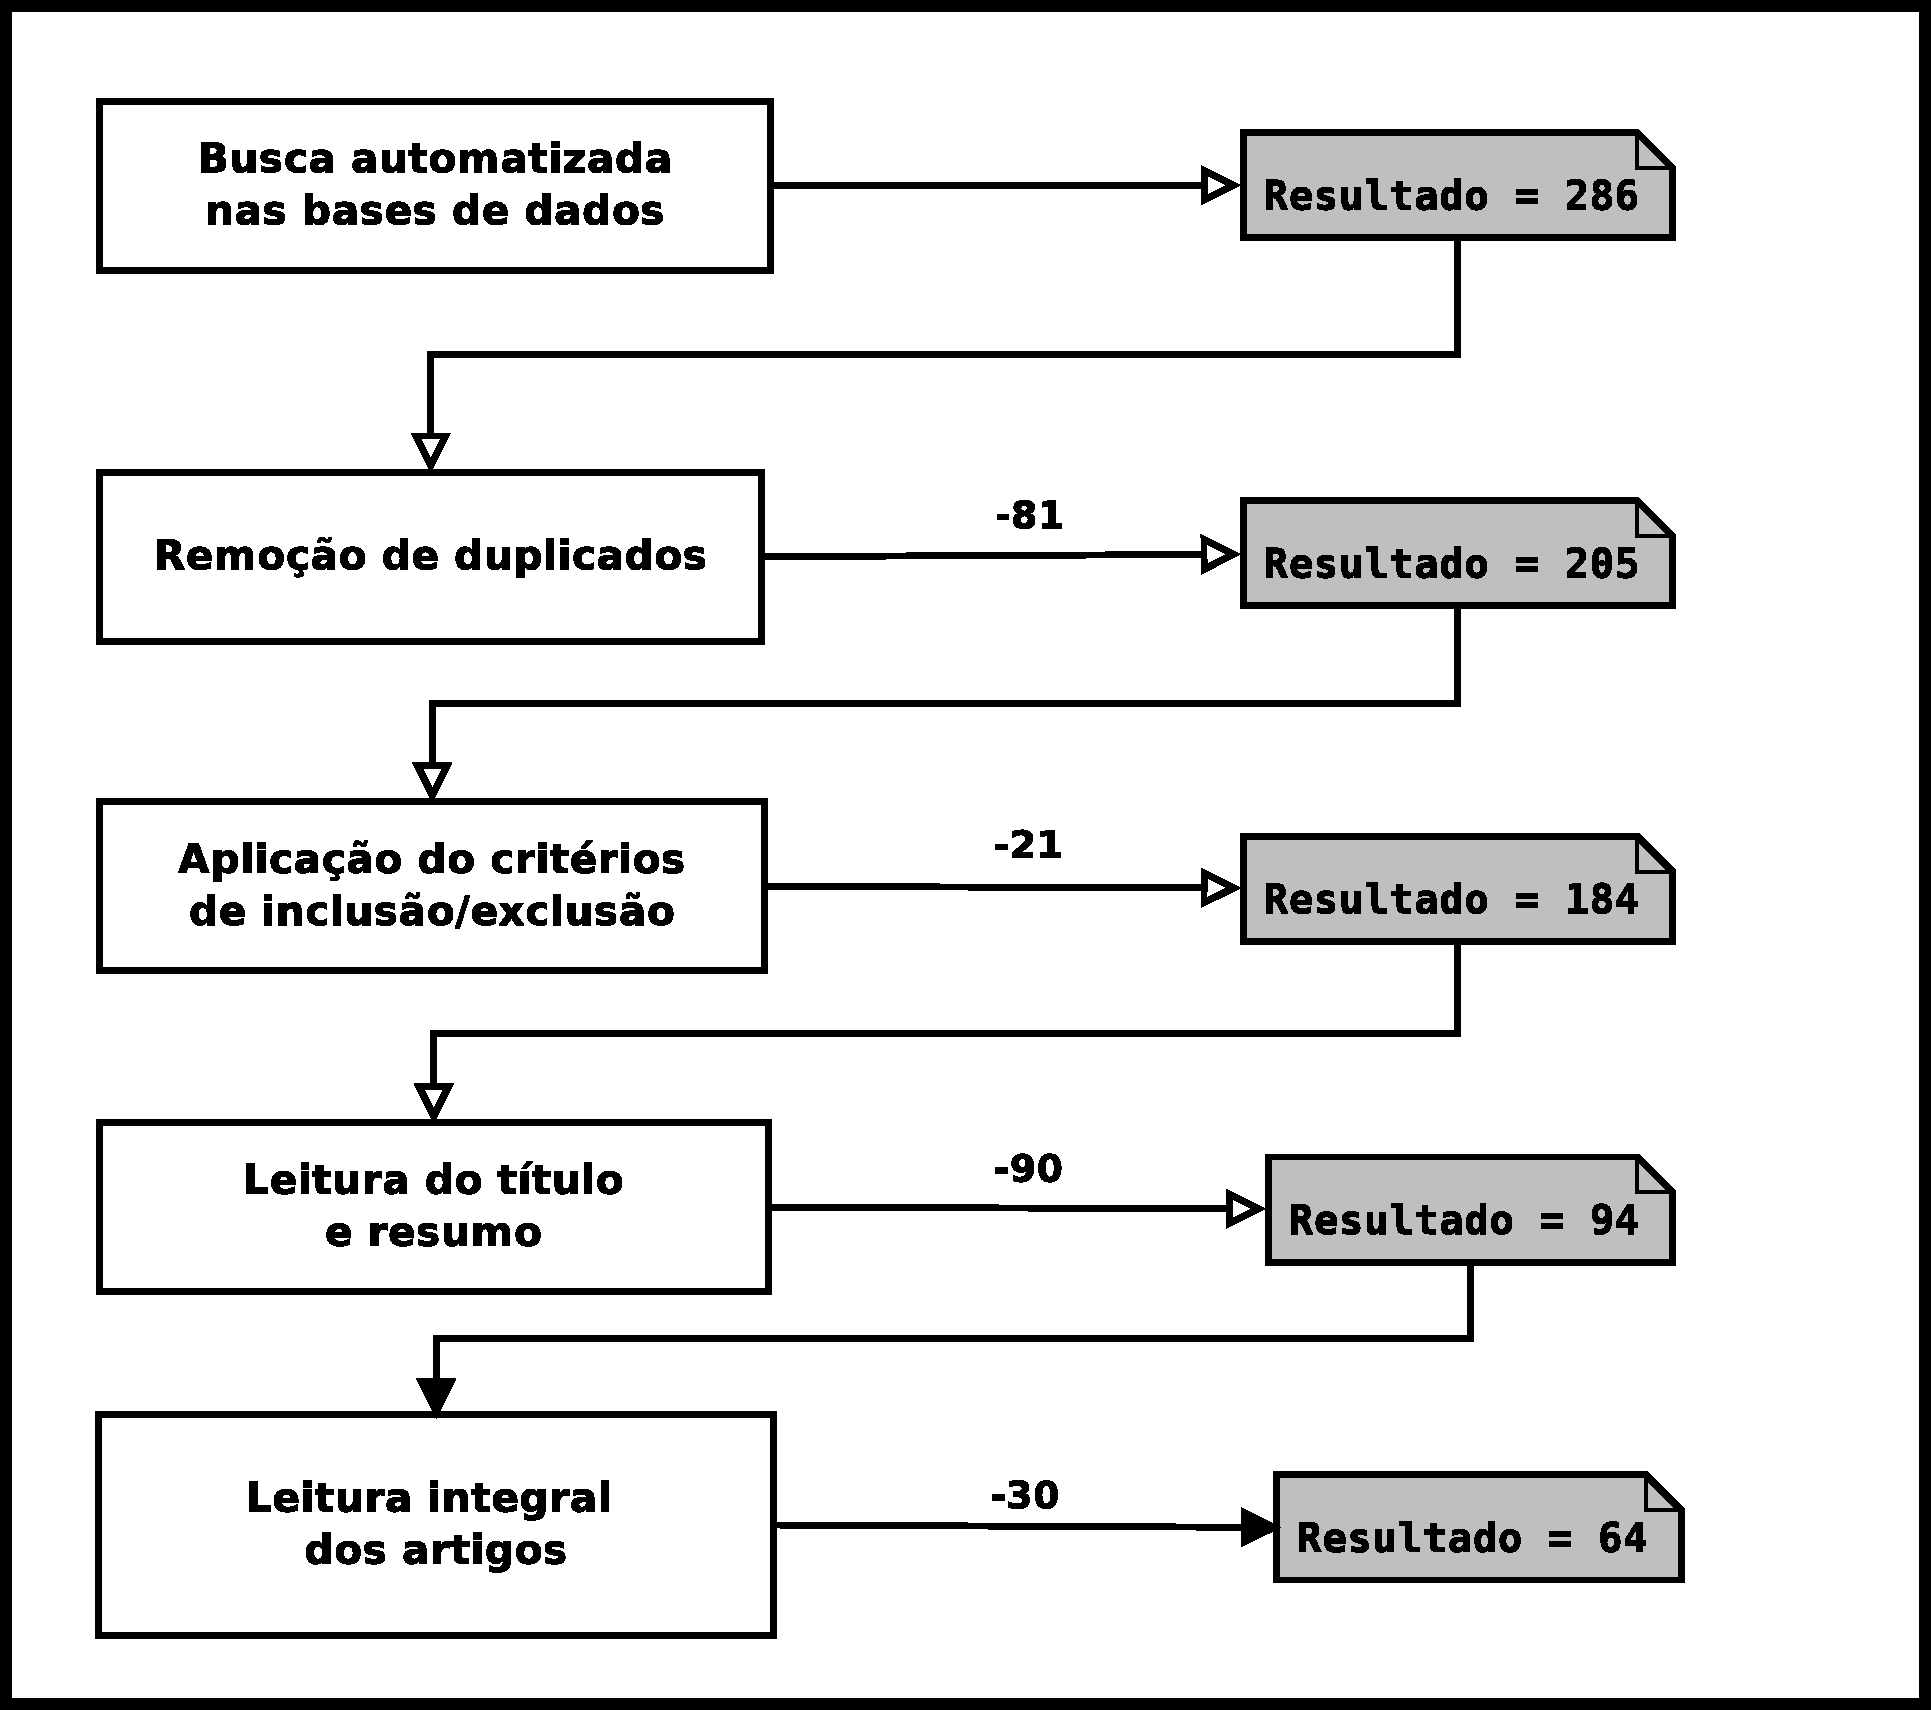
\includegraphics[width=0.75\linewidth]
	{./chapter-mapeamento-sistematico/img/diagrama-processo-selecao.pdf}
	\caption{Número de artigos incluídos durante o processo de seleção dos
		estudos. Baseado
		em~\cite{Petersen2015}}\label{fig:diagrama-processo-selecao}
\end{figure}

\begin{table}[htb] \centering \caption{Número de Estudos Recuperados por Base de
		Dados}\label{tab:estudos-por-base-dados} \begin{tabular}{cc} \hline
		\textbf{Base de Dados} & \textbf{Total} \\ \hline ACM Digital Library
		& 109            \\ IEEE Explore           & 100            \\
		Inspec/Compendex       & 22             \\ Scopus                 & 55
		\\ \hline \end{tabular}

\end{table}

\subsection{Esquemas de Classificação}
\label{subsec:map-esquemas-classificacao}

O mapeamento foi conduzido utilizado dois esquemas de classificação. O primeiro
organiza os artigos pela dimensão de melhoria que a funcionalidade que está
sendo proposta pertence. As dimensão de melhorias foram baseados no trabalho de
Zimmermann e outros e visam aperfeiçoar as funcionalidades das FGRM's de maneira
integral~\cite{zimmermann2009improving}. A segunda classificação distribuí os
estudos pelo suporte que é dado a determinado papel no processo de manutenção de
software. Entendemos que estes dois esquemas de classificação nos fornecem uma
visão de como as melhorias das funcionalidades vêm sendo propostas tanto do
ponto de vista de quem desenvolve quanto das diferentes partes interessadas
envolvidas nos projetos de software. As próximas subseções discutem em maior
detalhe os esquemas de classificação utilizados.

\subsubsection{Classificação por Dimensão de Melhoria}
\label{subsubsec:map-esquema-suporte-problema}

%Existem diversos problemas relacionados ao processo de Manutenção de Software.
%Já na década de 1980 algumas pesquisas questionavam os profissionais envolvidos
%com manutenção de software sobre quais os principais problemas da
%área\cite{Lientz:1981:PAS:358790.358796}. Naturalmente a percepção dos desafios
%envolvidos com a manutenção de software se altera com tempo, desta forma, é
%sempre válido revisar a literatura com o objetivo de entender como as
%funcionalidades oferecidas pelas FGRM estão dando suporte na resolução de tais
%problemas. Neste sentido foi proposto um esquema de classificação que relaciona
%os estudos com a dimensão de melhoria no qual a funcionalidade proposta visa
%solucionar.

Em um estudo sobre o aperfeiçoamento das FGRM's Zimmermann e outros argumentam
que ter informações completas nos relatos de bugs (Requisição de Mudança) tão
logo quanto possível ajuda os desenvolvedores a resolver rapidamente o
problema~\cite{zimmermann2009improving}. Neste estudo eles discutem dimensões de
melhorias que podem melhorar as funcionalidades oferecidas pelas FGRM's de forma
integral, ou seja, que atenda aos diversos contextos que este tipo software está
integrado.

\begin{description}
	\item[Foco na Informação] Estas melhorias focam diretamente na informação
		fornecida pelo reportador da RM\@. Com ajuda da FGRM o responsável por
		descrever um bug, por exemplo, poderia ser motivado a coletar mais
		informações sobre o problema. O sistema poderia verificar a validade e
		consistência daquilo que foi repassado pelo usuário.
   \item[Foco no Processo] Melhorias com foco no processo suporte atividade de
	   administração focadas na solução das RM's. Por exemplo,
	   a triagem de RM, poderia ser automatizada visando acelerar o processo. Um
	   outro exemplo de melhoria poderia ocorrer no aumento do entendimento do
	   progresso realizado em cada RM ou mesmo fornecer ao usuário afetado uma
	   estimativa do tempo de atendimento de uma requisição.
   \item[Foco no Usuário] Nesta dimensão estão incluídos tanto os usuário que
	   relatam as RM's quanto os desenvolvedores responsáveis por solucioná-la.
	   Os reportadores podem ser educados de qual informação fornecer e como
	   coletá-la. Os desenvolvedores também podem beneficiar de um treinamento
	   similar em qual informação esperar e como esta informação pode ser
	   utilizada para solucionar a RM\@.
	\item[Foco na Ferramenta] As melhorias centradas na ferramenta são
		realizadas nas funcionalidades fornecidas pelas FGRM\@. Elas podem
		reduzir a complexidade da coleta e fornecimento das informações
		necessárias para solucionar a RM\@. Por exemplo, as FGRM poderiam ser
		configuradas para automaticamente identificar a cadeia de registros de
		ativação de funções (stack trace) e adicioná-la ao erro reportado. A
		ferramenta poderia simplificar o processo de reprodução do erro mediante
		a captura automatizada de tela.Estes exemplos visam
		ajudar com a coleta das informações necessárias pelos desenvolvedores
		para corrigir o bug, por exemplo.
\end{description}

\begin{figure}[htpb] \centering
	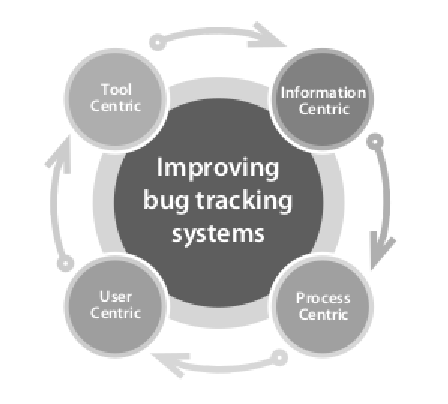
\includegraphics[width=0.666666\linewidth]
	{chapter-intro/img/dimensoes_melhorias_fgrm.pdf}
	\caption{Dimensões de melhoria das FGRM's. Adaptado
		de~\cite{zimmermann2005mining}}\label{fig:dimensoes_melhorias_fgrm}
\end{figure}

Para a classificação dos estudos foi realizado um processo com base em Petersen
e outros~\cite{Petersen2008}, compreendendo de duas etapas:

\begin{enumerate}[I]
	\item análise das palavras-chaves e conceitos que
		identificam as contribuições do estudo por meio da analise do título e
		resumo.
	\item combinações das palavras-chaves para construir um conjunto de
		categorias para classificação dos artigos.
\end{enumerate}

Os autores recomendam que nos casos em que o resumo e o título do estudo não
sejam capazes de caracterizá-lo, as seções de introdução e conclusão também
devem ser analisadas. Para as bases de dados onde era informado mais de um
conjunto de palavras-chaves para um mesmo artigo, utilizamos aquelas que foram
informadas pelos autores. Mediante a aplicação do processo foi construído o
esquema de classificação apresentado na
Figura~\ref{fig:diagrama-esquema-dimensao-melhorias}.

%\begin{figure}[tb] \centering
	%\makebox[\textwidth]{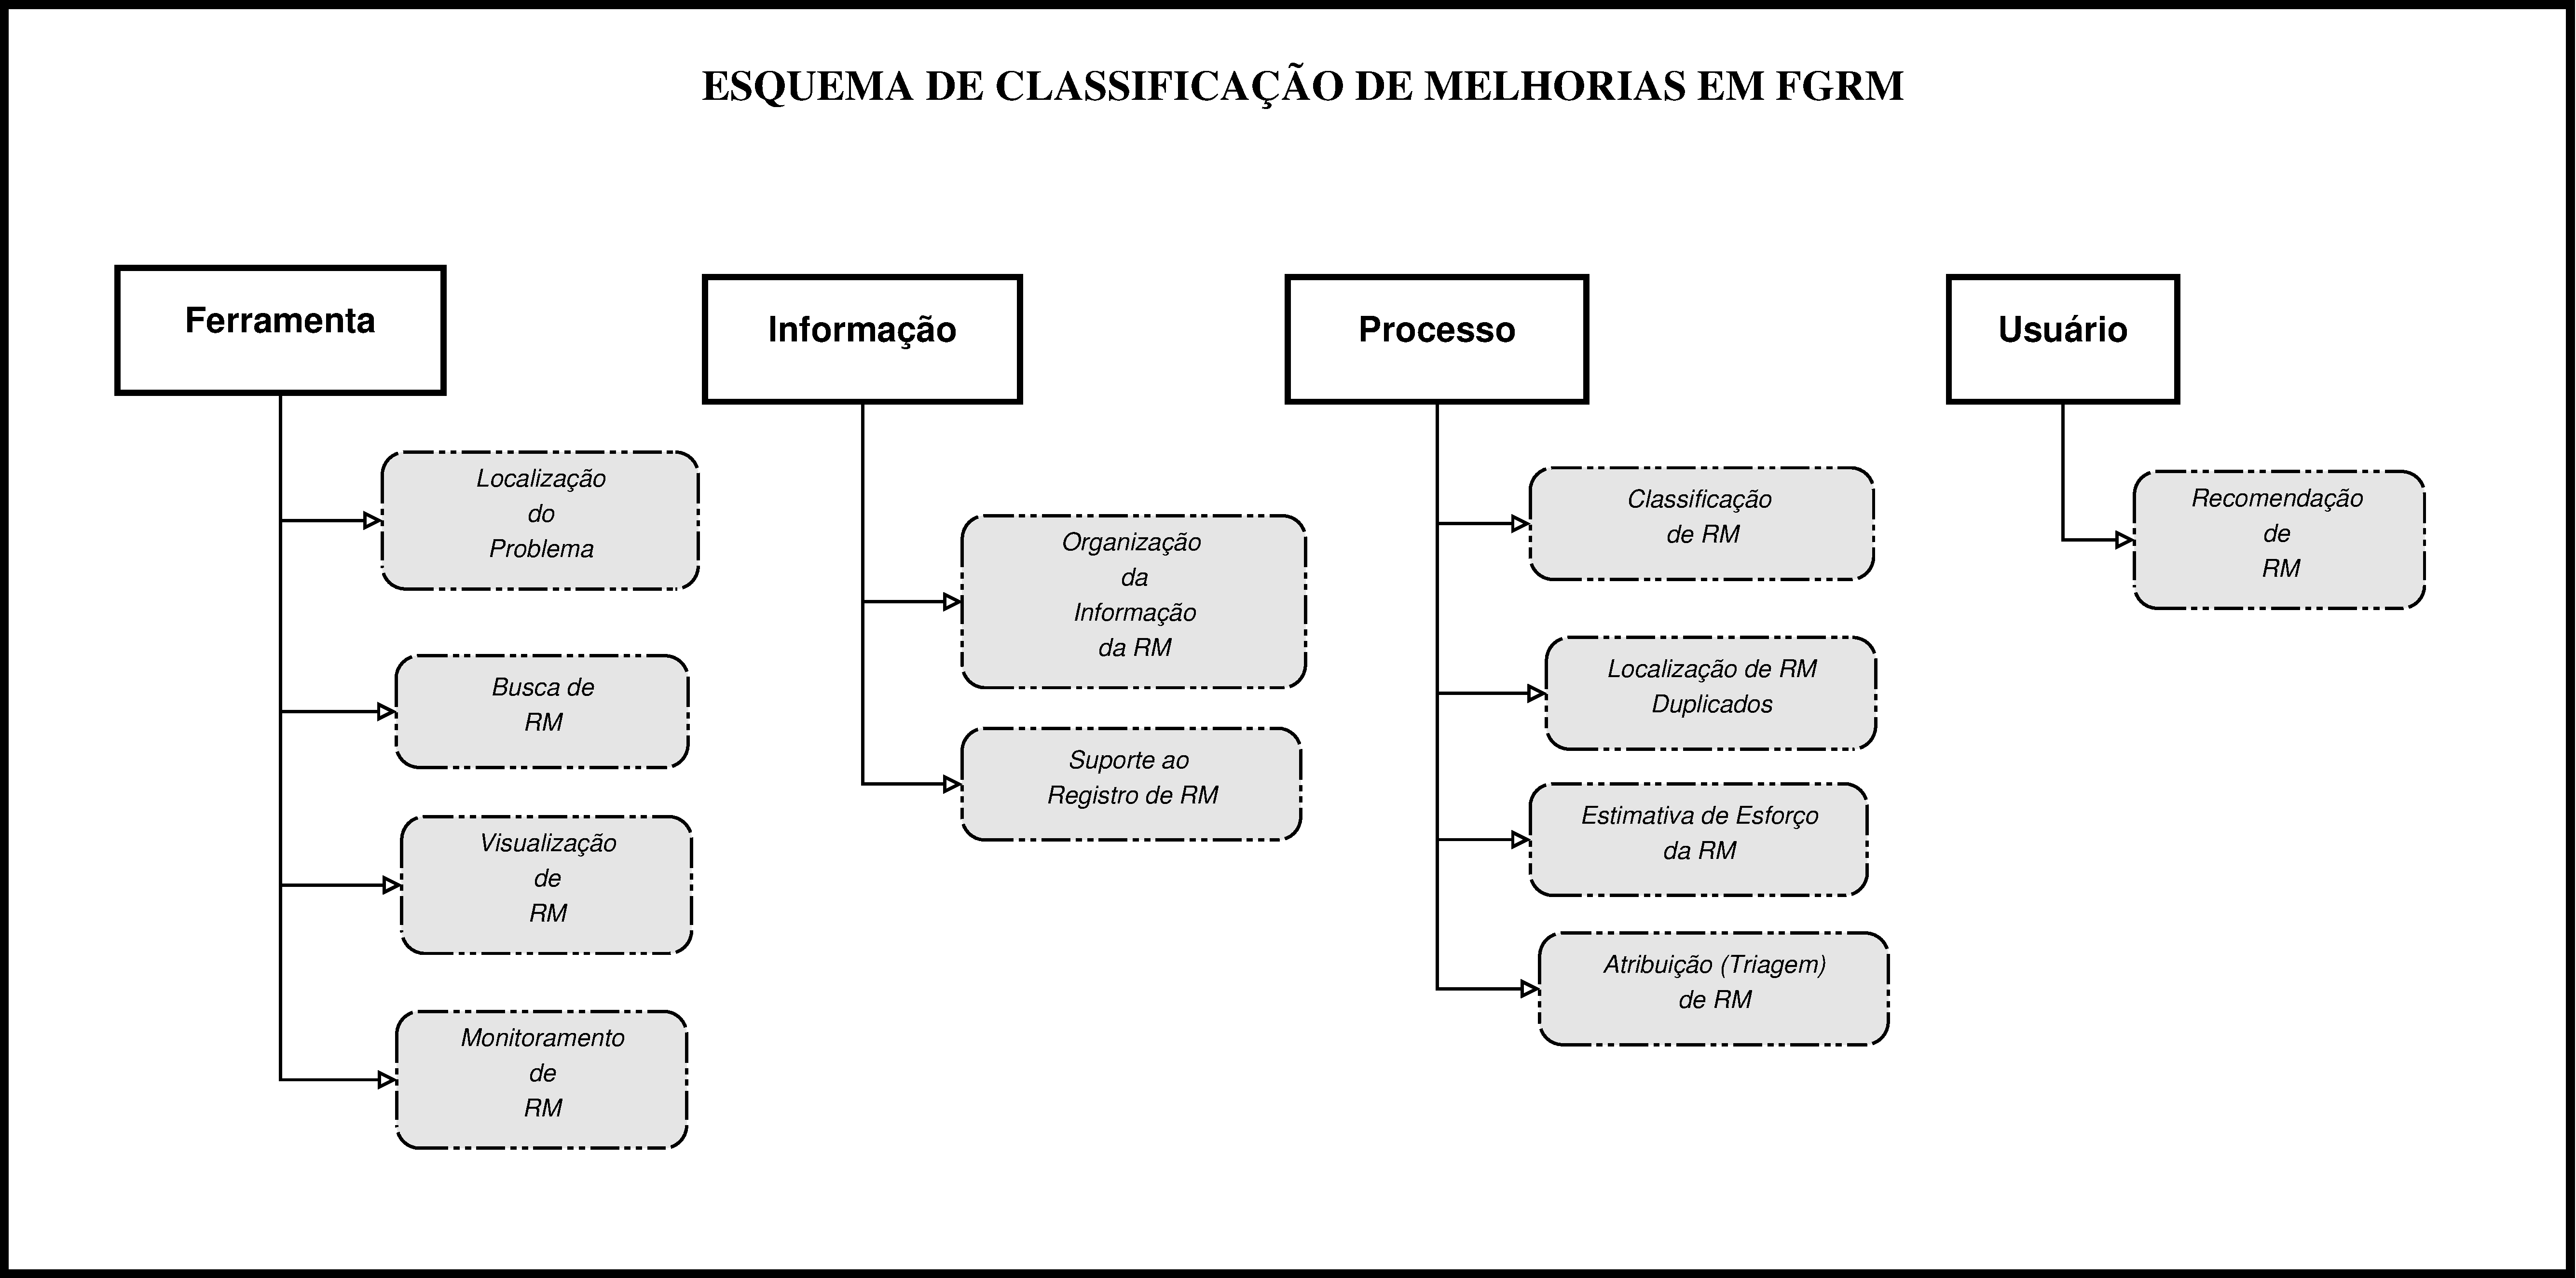
\includegraphics[width=.9\paperwidth]{./chapter-mapeamento-sistematico/img/diagrama-esquema-dimensoes-melhorias.pdf}}
	%\caption{Esquema de classificação das melhorias propostas na literatura. Os
		%retângulos representam as dimensões de melhorias e os polígonos de
		%cantos arredondados representam as melhorias.}
%\label{fig:diagrama-esquema-dimensao-melhorias}
 %\end{figure}

\subsubsection{Classificação por Suporte ao Papel da Manutenção de Software}
\label{subsubsec:map-esquema-suporte-papel-man}

Da mesma forma que uma funcionalidade proposta em determinado estudo visa
resolver algum problema da gestão das RM's, é possível supor que o foco de
alguns estudos pode estar relacionado com o suporte a alguns papeis
desempenhados no processo de Manutenção de Software. Este é o nosso segundo
esquema de classificação que utiliza os papéis descritos na
Subseção~\ref{subsec:man_visao_geral_papeis_na_manutencao_de_software}. A partir
desta classificação é possível verificar como os estudos escolhidos estão
distribuídos entre os diversos papéis, de modo avaliar os que recebem mais ou
menos atenção.

\section{Resultados}
\label{sec:mapeamento_resultados}

Nesta seção apresentamos para cada classificação os estudo que as compõem.
Iniciamos com uma análise da frequência de publicação relativo à melhoria das
funcionalidades das ferramentas. Posteriormente apresentamos os resultados pela
classificação por problemas na Manutenção de Software, o qual dividimos os
estudos por área e tópico de pesquisa. Seguimos com a análise dos estudos pelo
papel ao qual a funcionalidade proposta visa dar suporte.

\subsection{Frequência das Publicações}
\label{sub:frequencia_publicacao}

A Figura~\ref{fig:publicacao_por_ano} exibe o número de estudos primários
identificados entre os anos 2010\@-\@2016, período de referência utilizado no
mapeamento. Dentre os estudos escolhidos no período em questão verificamos que
em 2010 foram publicados cinco estudos sobre o
assunto~\cite{sun2010discriminative,gegick2010identifying,song2010jdf,nagwani2010predictive,zimmermann2010makes}.
Posteriormente verificamos um acréscimo no número de estudos no qual um
significante aumento pode ser observado entre os anos de 2012\@-\@2014.

\begin{figure}[htpb] \centering
	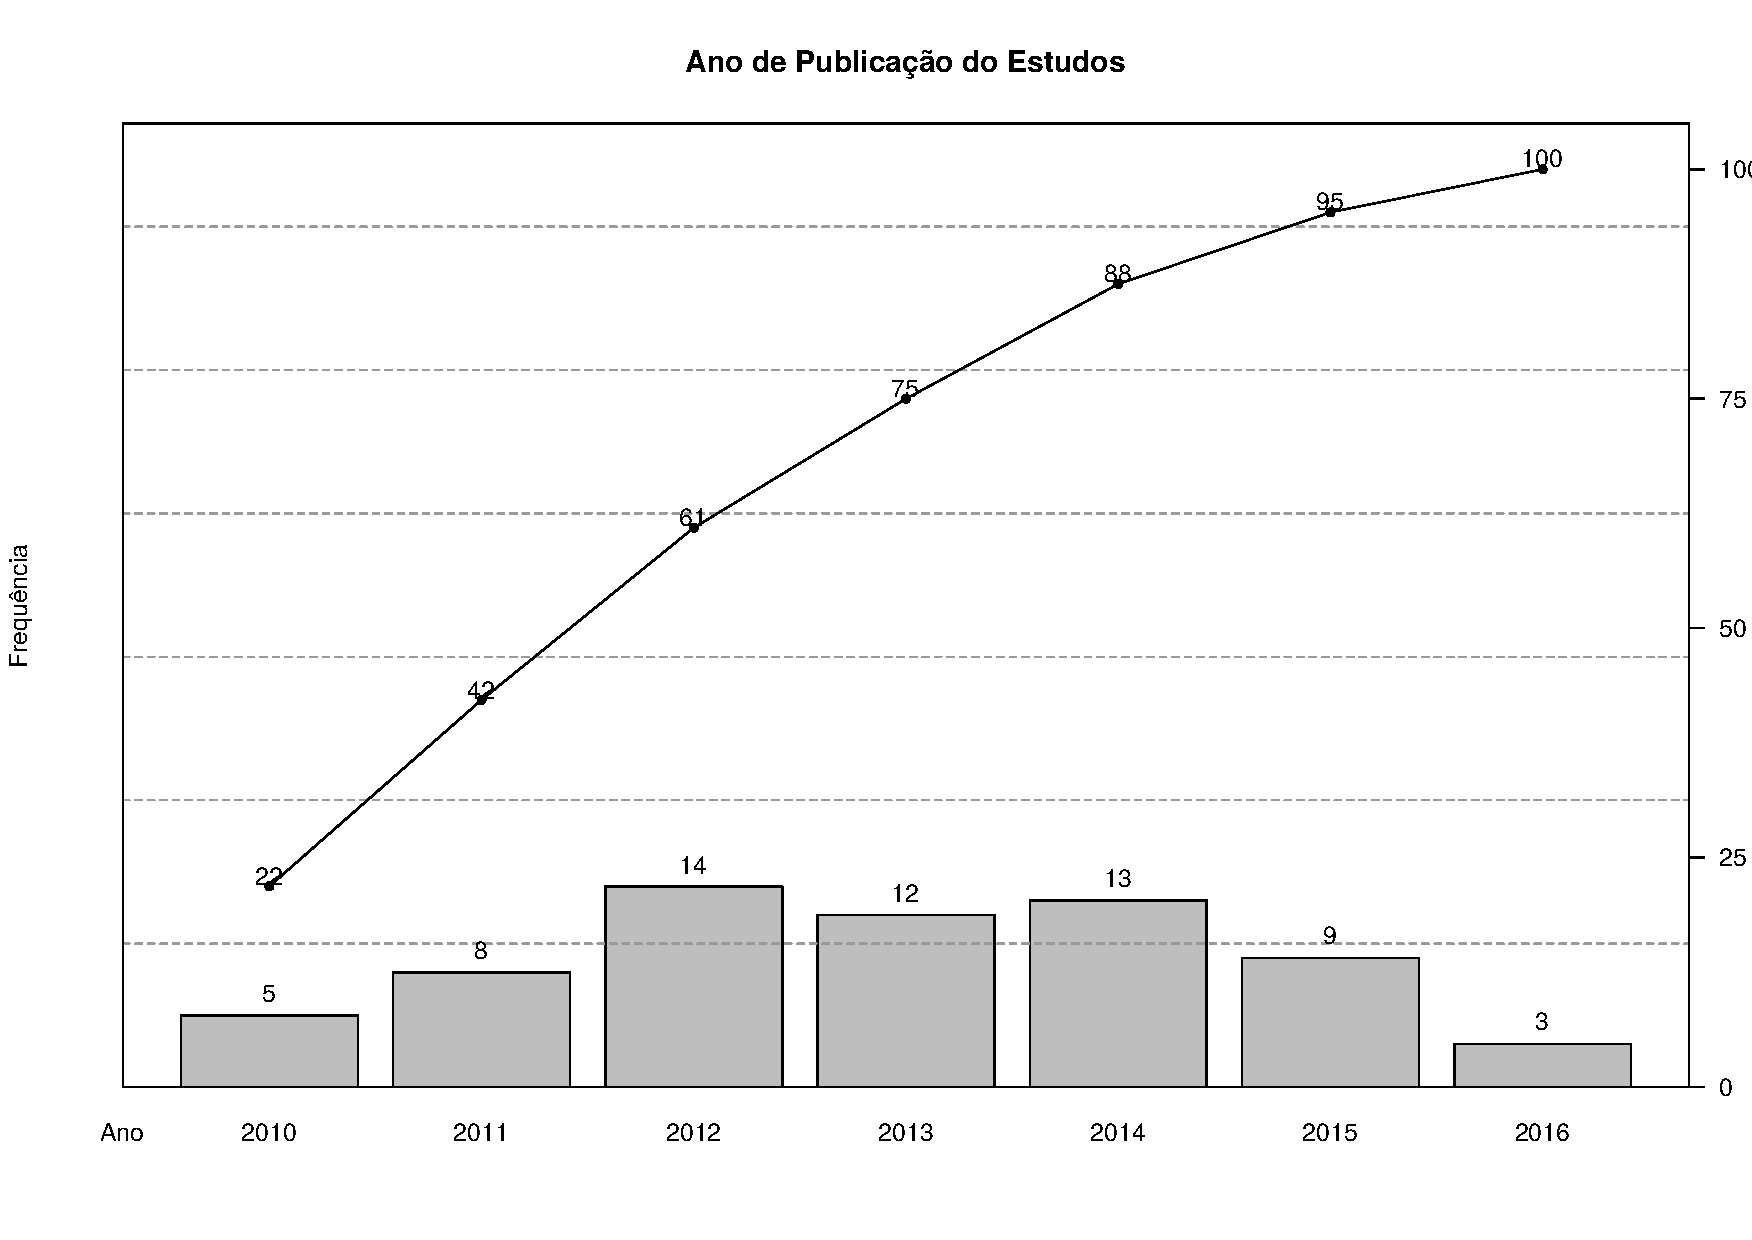
\includegraphics[width=0.9\linewidth]{chapter-mapeamento-sistematico/img/ano-publicao-estudos.pdf}
	\caption{Número de estudos primários por ano de publicação.}
\label{fig:publicacao_por_ano} \end{figure}

\subsection{Extensões para Problemas na Manutenção de Software}
\label{sub:extensões_para_problemas_na_manutenção_de_software}

Nesta parte do trabalho estamos interessados em caracterizar o estado da arte do
estudo dos problemas encontrados na Manutenção de Software relacionados à gestão
das RM's. Nesta seção apresentamos as funcionalidades das FGRM estão sendo
proposta na literatura. Adicionalmente a
Tabela~\ref{tab:taxonomia-problemas-manutencao} exibe a distribuição dos estudos
pela dimensão de melhoria e o seu respectivo tópico.

% Inclusão da tabela
\begin{table}[htbp]
\centering
\caption{My caption}
\label{my-label}
\resizebox{\textwidth}{!}{%
\begin{tabular}{|c|l|l|c|}
\hline
\textbf{Dimensão da Melhoria} & \multicolumn{1}{c|}{\textbf{Tópico}}             & \multicolumn{1}{c|}{\textbf{Estudos}}          & \textbf{Total}       \\ \hline
\multirow{13}{*}{Ferramenta}  & Busca de RM                                      & \cite{Liu2014}                                 & 1                    \\ \cline{2-4} 
                              & \multirow{7}{*}{Localização do Problema}         & \cite{Bangcharoensap:2012:LSC:2419061.2419428} & \multirow{7}{*}{7}   \\
                              &                                                  & \cite{Corley2011}                              &                      \\
                              &                                                  & \cite{Nguyen:2012:MAR:2393596.2393671}         &                      \\
                              &                                                  & \cite{Romo:2015:TAT:2745802.2745833}           &                      \\
                              &                                                  & \cite{thung2013automatic}                      &                      \\
                              &                                                  & \cite{Thung:2014:BIT:2635868.2661678}          &                      \\
                              &                                                  & \cite{Wong:2014:BBF:2705615.2706096}           &                      \\ \cline{2-4} 
                              & Monitoramento de RM                              & \cite{Aggarwal:2014:MIT:2593801.2593810}       & 1                    \\ \cline{2-4} 
                              & \multirow{4}{*}{Visualização de RM}              & \cite{dal2013closer}                           & \multirow{4}{*}{4}   \\
                              &                                                  & \cite{Hora2012}                                &                      \\
                              &                                                  & \cite{Sasso2014}                               &                      \\
                              &                                                  & \cite{takama2013application}                   &                      \\ \hline
\multirow{9}{*}{Informação}   & \multirow{2}{*}{Organização da Informação da RM} & \cite{mani2012ausum}                           & \multirow{2}{*}{2}   \\
                              &                                                  & \cite{Otoom2016}                               &                      \\ \cline{2-4} 
                              & \multirow{7}{*}{Suporte ao Registro da RM}       & \cite{Bettenburg2008a}                         & \multirow{7}{*}{7}   \\
                              &                                                  & \cite{Correa2013b}                             &                      \\
                              &                                                  & \cite{moran2015auto}                           &                      \\
                              &                                                  & \cite{Moran:2015:EAA:2786805.2807557}          &                      \\
                              &                                                  & \cite{Tu:2014:MQI:2677832.2677844}             &                      \\
                              &                                                  & \cite{White:2015:GRR:2820282.2820291}          &                      \\
                              &                                                  & \cite{Wu2011a}                                 &                      \\ \hline
\multirow{40}{*}{Processo}    & \multirow{12}{*}{Atribuição (Triagem) de RM}     & \cite{Banitaan2013}                            & \multirow{12}{*}{12} \\
                              &                                                  & \cite{hosseini2012market}                      &                      \\
                              &                                                  & \cite{Hu:2014:EBT:2707683.2708297}             &                      \\
                              &                                                  & \cite{Naguib2013}                              &                      \\
                              &                                                  & \cite{Nagwani2012}                             &                      \\
                              &                                                  & \cite{shokripour2012automatic}                 &                      \\
                              &                                                  & \cite{tian2015automated}                       &                      \\
                              &                                                  & \cite{ValdiviaGarcia:2014:CPB:2597073.2597099} &                      \\
                              &                                                  & \cite{Wu2011}                                  &                      \\
                              &                                                  & \cite{Xuan:2012:DPB:2337223.2337227}           &                      \\
                              &                                                  & \cite{Zanetti2013}                             &                      \\
                              &                                                  & \cite{Zhang2014}                               &                      \\ \cline{2-4} 
                              & \multirow{10}{*}{Classificação de RM}            & \cite{behl2014bug}                             & \multirow{10}{*}{10} \\
                              &                                                  & \cite{chawla2015automated}                     &                      \\
                              &                                                  & \cite{Gegick2010}                              &                      \\
                              &                                                  & \cite{Izquierdo2015}                           &                      \\
                              &                                                  & \cite{kochhar2014automatic}                    &                      \\
                              &                                                  & \cite{Nagwani2013}                             &                      \\
                              &                                                  & \cite{netto2010automated}                      &                      \\
                              &                                                  & \cite{somasundaram2012automatic}               &                      \\
                              &                                                  & \cite{Tian:2013:DPP:2550526.2550574}           &                      \\
                              &                                                  & \cite{zhang2011bug}                            &                      \\ \cline{2-4} 
                              & \multirow{5}{*}{Estima de Esforço da RM}         & \cite{Bhattacharya:2011:BTP:1985441.1985472}   & \multirow{5}{*}{5}   \\
                              &                                                  & \cite{Nagwani2010}                             &                      \\
                              &                                                  & \cite{Thung2012}                               &                      \\
                              &                                                  & \cite{Vijayakumar2014}                         &                      \\
                              &                                                  & \cite{xia2015automatic}                        &                      \\ \cline{2-4} 
                              & \multirow{13}{*}{Localização de RM Duplicados}   & \cite{alipour2013contextual}                   & \multirow{13}{*}{13} \\
                              &                                                  & \cite{banerjee2012automated}                   &                      \\
                              &                                                  & \cite{hindle2016contextual}                    &                      \\
                              &                                                  & \cite{Koopaei:2015:CAD:2886444.2886474}        &                      \\
                              &                                                  & \cite{Lerch:2013:FDY:2495256.2495763}          &                      \\
                              &                                                  & \cite{Liu:2012:TBR:2393596.2393628}            &                      \\
                              &                                                  & \cite{Prifti2011}                              &                      \\
                              &                                                  & \cite{Song2010a}                               &                      \\
                              &                                                  & \cite{sun2010discriminative}                   &                      \\
                              &                                                  & \cite{Sun2011}                                 &                      \\
                              &                                                  & \cite{Thung2014}                               &                      \\
                              &                                                  & \cite{Tian2012}                                &                      \\
                              &                                                  & \cite{Tomasev2013}                             &                      \\ \hline
\multirow{2}{*}{Usuário}      & \multirow{2}{*}{Recomendação de RM}              & \cite{malheiros2012source}                     & \multirow{2}{*}{2}   \\
                              &                                                  & \cite{Wang2011a}                               &                      \\ \hline
\end{tabular}%
}
\end{table}


\begin{figure}[tb] \centering
	\makebox[\textwidth]{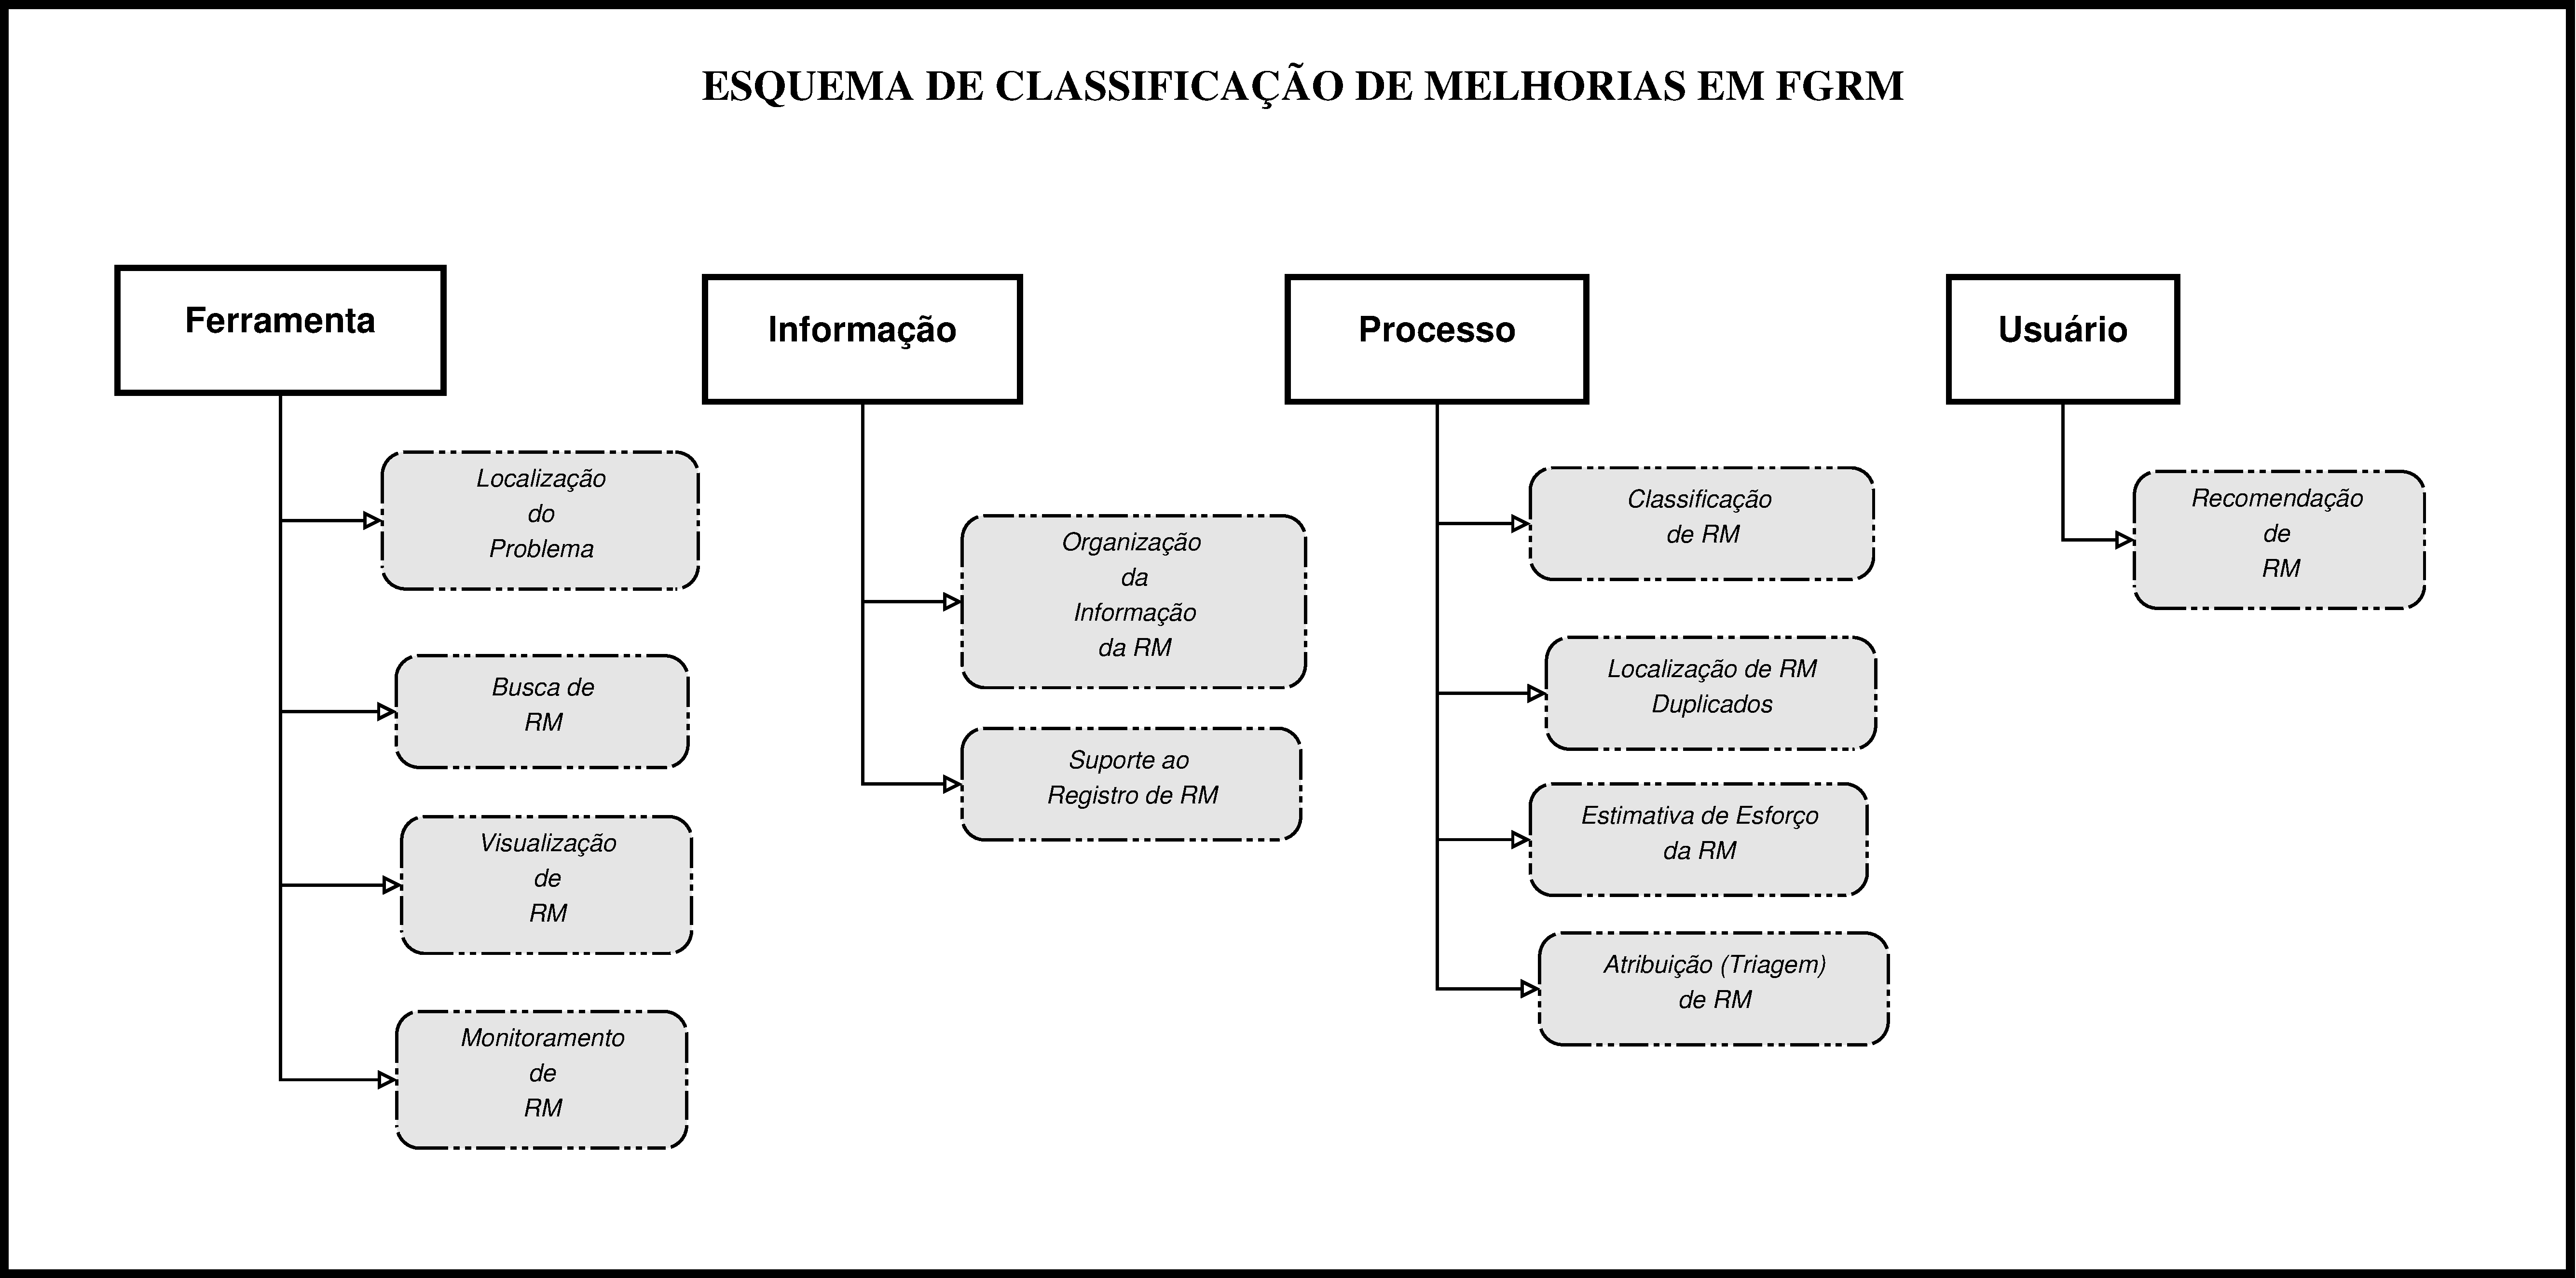
\includegraphics[width=.9\paperwidth]{./chapter-mapeamento-sistematico/img/diagrama-esquema-dimensoes-melhorias.pdf}}
	\caption{Esquema de classificação das melhorias propostas na literatura. Os
		retângulos representam as dimensões de melhorias e os polígonos de
		cantos arredondados representam as melhorias.}
	\label{fig:diagrama-esquema-dimensao-melhorias} \end{figure}

\todobegin{Trocar figura por tabela}
\begin{figure}[htpb] \centering
	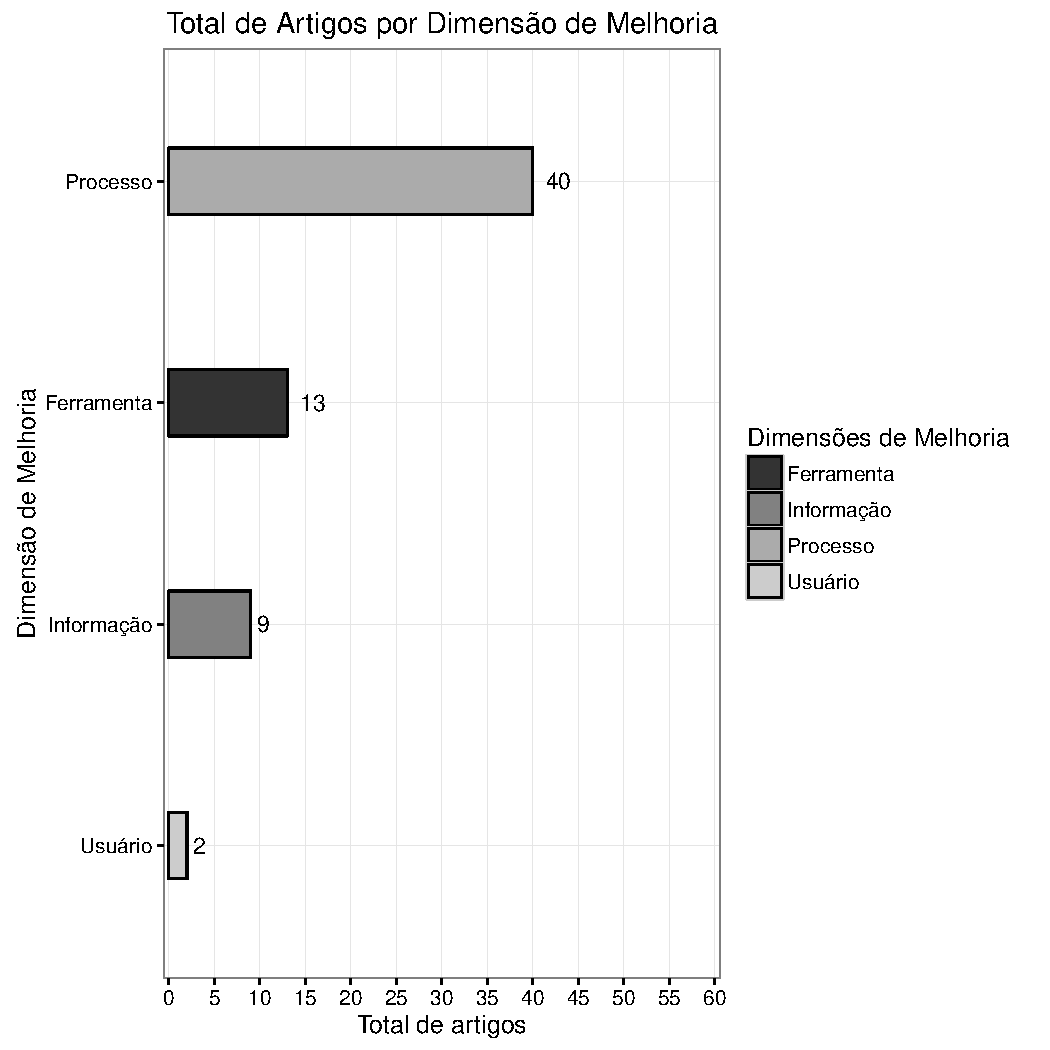
\includegraphics[width=0.9\linewidth]{./chapter-mapeamento-sistematico/img/grafico_dim_melhoria_por_artigo.pdf}
	\caption{Total de artigos por dimensão de melhoria}
	\label{fig:grafico_dim_melhoria_por_artigo} \end{figure}

\begin{figure}[htpb] \centering
	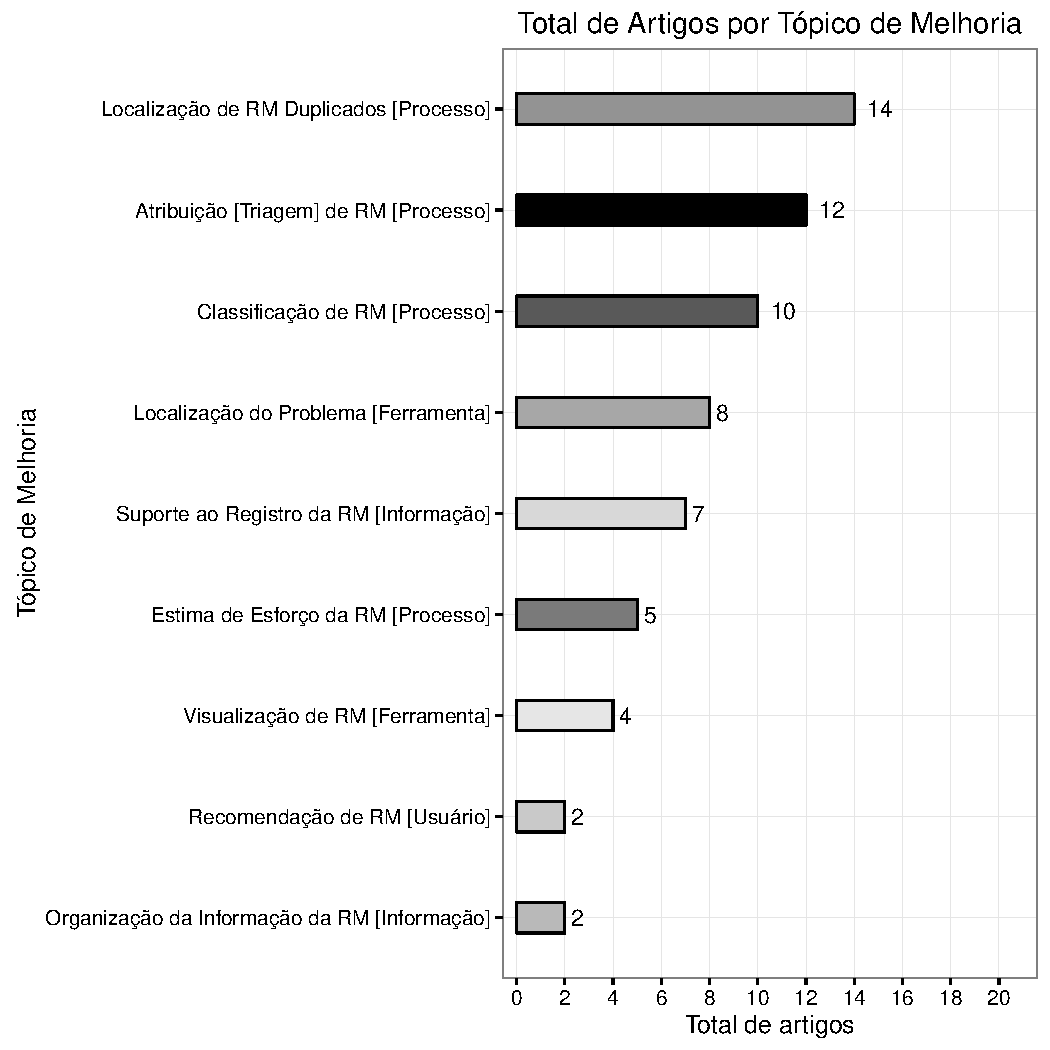
\includegraphics[width=0.8\linewidth]{./chapter-mapeamento-sistematico/img/grafico_topico_por_artigo.pdf}
	\caption{Total de artigos por tópico de melhoria}
	\label{fig:grafico_topico_por_artigo} \end{figure}

\subsubsection{Melhorias Propostas na Dimensão Ferramenta}
\label{ssub:melhorias_dim_ferramenta}

Este ramo do esquema de classificação proposto foi criado para classificar os
estudos que discutem melhorias na dimensão Ferramenta. Conforme anteriormente
exposto, esta classe acomoda estudos em tópicos como Localização do Problema e
Visualização de RM's.

\paragraph{Localização do Problema} Os estudos incluídos neste tópico de
classificação focam no problema de localizar a origem de um problema de software
com base dos dados da RM\@. Trata-se do processo de estatisticamente localizar
um bug utilizando os dados das RM's em conjunto com o código
fonte~\cite{Hovemeyer:2004:FBE:1052883.1052895}.

A tarefa de encontrar a origem de uma falha de software é complexa e consome
muito tempo. Em um estudo Lúcia e outros relataram que entre 84 a 93\% de
problemas em software afetam apenas 1~-~2 arquivos de
código-fonte~\cite{thung2012faults}. Contudo não é fácil identificar esses
poucos arquivos entre os milhares de arquivos de código-fonte. Esta situação
realça que localizar a origem de um problema (buggy files) é uma tarefa
árdua~\cite{Thung:2014:BIT:2635868.2661678}.

Neste contexto, pesquisadores vêm propondo abordagens baseadas em Recuperação da
Informação para localizar falhas com base no que está descritos nos relatos de
defeitos. Nessas abordagens existe a tentativa de encontrar entre o código fonte
do sistema um subconjunto de arquivos do código fonte que estão diretamente
relacionados à solução do problema
reportado~\cite{Wong:2014:BBF:2705615.2706096}.

Com objetivo de melhorar a eficiência da Localização do Problema diversas
informações contidas nas RM's estão sendo utilizadas. As diversas abordagens
propostas utilizam informações como cadeia de registros de ativação de funções
(stack-trace)~\cite{Wong:2014:BBF:2705615.2706096}, des\-cri\-ção e campos
estruturados das RM's~\cite{Thung:2014:BIT:2635868.2661678}, o históricos de
versões~\cite{Bangcharoensap:2012:LSC:2419061.2419428,corley2011recovering,Romo:2015:TAT:2745802.2745833}.

Alguns dos estudos propostos foram incluídos em ferramentas largamente
empregadas no mercado utilizando as propriedades de extensão do
software~\cite{Thung:2014:BIT:2635868.2661678,corley2011recovering}. Os autores
argumentam que pelo fato de nenhuma das técnicas propostas na literatura estarem
integradas às FGRM existe uma dificuldade de adoção da prática da localização
automática de problemas pelos desenvolvedores. Neste sentido, eles argumentam
sobre a necessidade da melhoria das funcionalidades das FGRM em especial com
melhoria ou inclusão de funcionalidades nas FGRM's utilizando o que vem sendo
proposto na literatura.

\paragraph{Visualização de RM} Os estudos classificados neste tópicos propõem
melhorar a visualização das informações contidas em uma RM\@. A tomada de
decisão deve estar subsidiada por informações corretas. Este fato não é
diferente na manutenção e desenvolvimento de software. Pouco se sabe sobre o
comportamento evolutivo, o tempo de vida, distribuição e estabilidade dos
problemas reportados nas FGRM~\cite{hora2012bug}. Este problema é reforçado pela
forma como as FGRM's armazenam os dados das RM's. Em geral, esses exibem
informações sobre as RM's de forma textual, o que não é apenas complicado para
navegar, mas também dificulta a compreensão das complexas peças de informação
que giram em torno dos problemas de software~\cite{dal2014bug}.

Com o objetivo de apresentar novas formas de visualizar os dados de uma RM novos
conceitos estão sendo propostos. No estudo de Hora e outros~\cite{hora2012bug} é
apresentado o conceito de Mapas de Bugs (Bugs Maps) que é a ligação de uma RM
com diversos outros artefatos de software como por exemplo o histórico de
versões.  No estudo de Lanza e  Dal Sasso~\cite{dal2014bug} o conceito de
hiperligação entre documentos é utilizado para permitir a navegação entre os
diversos artefatos que estão relacionados a um RM\@.

Por outro lado, verificamos o artigo proposto por Takama e
Kurosawa~\cite{takama2013application} onde a aplicação de tecnologias de
visualização de informação foi empregada para o monitoramento das informações
contidas nas RM's. A atualização das informações de uma RM quando gerenciada por
uma FGRM são estruturadas como cadeira de caracteres. Contudo, é difícil para as
partes interessadas monitorar uma RM o tempo todo. Neste contexto, a solução
proposta pelo autores visa suportar o monitoramento das RM apresentando ao
usuário mediante animações as atualizações ocorridas em determinada RM\@.

Por conta da natureza das melhorias propostas neste tópico de pesquisa,
verificamos que diversos estudos foram prototipados em ferramentas. Desta forma,
é possível avaliar as propostas através das ferramentas como o
bugMaps~\cite{hora2012bug} e In* Bug~\cite{dal2014bug}.

\subsubsection{Melhorias Propostas na Dimensão Informação}
\label{ssub:melhorias_dim_informacao}

Apresentamos aqui os trabalhos relacionados à melhoria da qualidade da
informação de uma RM.  A melhoria pode envolver suporte ao registro de uma RM
antes que ela seja armazenada na base de dados de uma FGRM\@; a melhoria também
pode envolver a organização da informação já registrada em uma RM, de modo a
facilitar o entendimento pelos desenvolvedores e demais profissionais envolvidos
na manutenção de software.

\paragraph{Suporte ao Registro da RM}

%Durante o processo de correção de um problema de software verifica-se que a
%reprodução manual dos bugs é demorada e tediosa
Os mantenedores de software rotineiramente tentam reproduzir problemas não
confirmados usando as informações contidas nas RM's que muitas vezes estão
incompletas~\cite{White:2015:GRR:2820282.2820291}. Para complementar os dados
necessários à resolução do problema o desenvolvedor deve solicitar ao
responsável pelo relato da RM as informações necessárias~\cite{5070993}. Os
relatos contidos nas RM's podem conter informações valiosas que podem ser
utilizadas para melhorar a qualidade da informação contidas em novos relatórios
de problemas de software. Esta melhoria da qualidade pode implicar na redução do
custo do processo de garantia de qualidade bem como aumentar a confiabilidade do
software com a redução gradativa de bugs~\cite{Tu:2014:MQI:2677832.2677844}.

A pesquisa visando a melhoria da qualidade da informação fornecida nas RM's
começa com estudos visando mensurar de alguma forma os relatos realizados pelos
usuários. A determinação do que seria um boa descrição de um problema de
software foi obtido mediante uma pesquisa (survey) com profissionais de
manutenção de software~\cite{Bettenburg2008a}. Em outro estudo os autores
propõem as métricas que posteriormente foram utilizadas para avaliar o relato
que compõe a RM~\cite{Tu:2014:MQI:2677832.2677844}.

Um segundo nicho de estudos  nesta área está relacionado ao suporte na
reprodução do erro do software. Estes estudos incluem tanto em registrar o
conjunto de ações que resultaram no erro~\cite{White:2015:GRR:2820282.2820291},
quanto em autocompletar as informações que compõe o relato do
problema~\cite{moran2015auto}. Um ponto em comum deste dois estudos é que eles
foram desenvolvido para o ambiente de desenvolvimento móvel, especial para o
sistema Android~\footnote{\url{https://www.android.com/}}. Uma possível
justificativa para este foco em aplicações móveis pode estar relacionado à
inerente dificuldade em registrar um problema de software naquele ambiente de
software.

Muitos dos estudos realizados resultaram em ferramentas com a finalidade de
realizar uma prova de conceito no tocante a dar suporte ao usuário em fornecer
um relato de boa qualidade~\cite{Tu:2014:MQI:2677832.2677844, Bettenburg2008a,
	Wu2011a,White:2015:GRR:2820282.2820291,moran2015auto}. 

\paragraph{Organização da Informação da RM}

Em alguns casos não é possível aumentar a qualidade da informação fornecida
em um relato de uma RM antes que ela seja armazenada em seu respectivo
repositório.  Nestas situações uma abordagem adotada é organizar de uma
maneira previamente definida as informações contidas em uma RM\@.

Durante o processo de análise de uma RM, em especial para aquelas de caráter
corretiva, existe a tendência dos desenvolvedores procurar por problemas
semelhantes que foram resolvidos no passado. No entanto, em diversas situações o
desenvolvedor precisar examinar manualmente o conteúdo dos bugs recomendados que
podem variar em tamanho e complexidade~\cite{mani2012ausum}.  Neste contexto, o
resumo (sumarização) automático de RM's que tenham relação com problema em
análise é uma maneira de reduzir a quantidade de dados que um desenvolvedor
precisa analisar. A ferramenta denominada AUSUM~\cite{mani2012ausum} propõe uma
abordagem, utilizando técnicas não supervisionadas de Recuperação da Informação,
de criar este resumo automático de um conjunto de relatos de problemas.

\subsubsection{Melhorias Propostas na Dimensão Processo}
\label{ssub:melhorias_dim_processo}

\todobegin{Foi realizada a alteração do foco da classificação, em que os estudos
são apresentados pela \textbf{forma} como ele trata o problema.}

\paragraph{Identificação de RM Duplicadas} O processo de identificação de RM's
duplicadas consiste em avaliar se determinado relato já foi realizado em algum
outro momento. A abordagem adotada da literatura para tratar o problema pode ser
dividida em dois tipos\cite{kaushik2012comparative, tian2012improved}:

\begin{enumerate}[(i)]
	\item remoção de duplicatas
	\item identificação de duplicatas
\end{enumerate}

No primeiro tipo, o objetivo é evitar que RM's duplicadas entrem na base de
dados de uma FGRM e desta forma evitar o esforço e o tempo extra necessário para
identificá-la posteriormente. Por outro lado, no segundo tipo o objetivo é
sugerir uma lista de possíveis duplicatas durante o processo de registro de uma
nova RM e possivelmente agrupá-los. Um ponto importante para se ressaltar é que
este segundo tipo se baseia na premissa que registrar um mesmo problema por mais
de uma vez nem sempre é problemático tendo em vista que pode fornecer
informações adicionais que podem ser úteis~\cite{bettenburg2008duplicate}. É
importante que novas abordagens tentem equilibrar este dois tipos de tratamento
de modo a evitar o tempo extra para análise de uma RM bem como apoiar os
desenvolvedores com informações
adicionais~\cite{Lerch:2013:FDY:2495256.2495763,Thung2014}.

Uma forma de tratar o problema é utilizar modelos de espaços vetoriais para
medir a similaridade entre as RM~\cite{liu2014faceted, sun2010discriminative,
	Thung2014,tomavsev2013exploiting}. Outros trabalhos tentam utilizar outras
técnicas que partem da premissa que os termos específicos de domínio contidos no
relato das RM's são essenciais na determinação da probabilidade de duas
requisições serem duplicadas~\cite{hindle2016contextual, alipour2013contextual}.
Em resumo verificamos que o relato contido na RM é utilizado com fonte primária
de informação para técnicas de Recuperação da Informação visando determinar a
similaridade entre duas RM's. A partir de medida encontrada é possível
determinar se as requisições referem-se ao mesmo pedido.

\todoend


\paragraph{Atribuição (Triagem) de RM} A atividade de atribuição de RM, que é a
principal atividade do processo conhecido como \textit{triagem}, possui como
principal objetivo encontrar o desenvolvedor mais capacitado para manipular uma
dada RM~\cite{cavalcanti2014challenges}. Existe a premissa de que a escolha do
desenvolvedor apropriado é crucial para obter em menor tempo a re\-so\-lu\-ção
de determinada RM~\cite{di2002approach}. Estudos também discutem que o processo
de atribuição deve considerar fatores tais como a carga de trabalho do
desenvolvedor a prioridade da RM~\cite{aljarah2011selecting}.

\todobegin{Revisar qual tipo de classificação está sendo realizada}
\paragraph{Classificação da RM} Independentemente do tipo e tamanho de um
projeto é sempre importante determinar qual tipo manutenção deverá ser realizada
tomando como base o relato de uma RM\@.  Este processo consiste de forma
resumida em classificar uma requisição com base em algum esquema de
classificação previamente definido. A diversidade de categorias em determinado
esquema de classificação pode tornar complexa a tarefa, tendo em vista que em
muitos casos não é fácil determinar os limites entre os
tipos~\cite{antoniol2008bug}. Por exemplo, a uma classificação incorreta de um
defeito como melhoria pode acarretar em atrasos no projeto ou mesmo que uma RM
receba pouca atenção~\cite{cavalcanti2014challenges}.

\paragraph{Estimativa de Esforço da RM} A gestão de custo e esforço de um
projeto de manutenção de software passa pelo controle do esforço necessário ao
cumprimento de suas RM's. Os estudos que tratam das questões de estimativa de
esforço requerido para a solução do problema descrito em uma RM utilizam em
geral três formas para estimá-lo~\cite{cavalcanti2014challenges}: determinar o
tempo para solucionar novas RM's; definir os artefatos que são impactados por
determinada RM\@; prever o número de novas RM's que poderão fazer parte do
projeto.

No primeiro tipo de estudo a preocupação é estimar o tempo necessário para
tratar a mudança solicitada em determinada requisição. Naturalmente, existe
certa complexidade em produzir uma estimativa precisa em função das diferentes
atividades envolvidas e também em função dos diferentes níveis de capacitação
que o responsável pela execução das tarefas pode ter~\cite{xia2015automatic}.
Apesar da inerente imprecisão deste tipo de trabalho é importante salientar que
estimar o tempo de solução de uma RM é importante para o gerenciamento do
projeto porque ajuda alocar recurso de forma mais
eficiente~\cite{Bhattacharya:2011:BTP:1985441.1985472} e melhorar a previsão do
custo necessário para o lançamento de futuras versões do
sistema~\cite{Vijayakumar2014}.

No segundo grupo temos os artigos que tentam identificar previamente o conjunto
de artefatos que serão impactados pela tarefa de manutenção~\cite{Nagwani2010}.
A literatura sobre análise de impacto é bastante abrangente e pode envolver o
estudos de artefatos tais como documentos de requisitos e arquiteturas de
softwares, código fonte, registros (logs) de teste e assim por
diante~\cite{cavalcanti2014challenges}. Neste sentido, estamos focados em
estudos onde as RM's são o ponto de partida para a análise de impacto. O último
grupo de estudos discutem técnicas sobre como prever o número de RM's que
possivelmente serão relatadas em futuras versões do sistema. De forma similar ao
primeiro grupo este tipo de estudo visa contribuir com o planejamento das
atividades de manutenção e evolução. A predição do que será relatado incluí RM's
que não existiam em versões anteriores, por exemplo, bem como aqueles que serão
reabertos, ou seja, problemas que não foram solucionados anteriormente mesmo as
suas RM's dizendo o contrário~\cite{xia2015automatic}.

\subsubsection{Melhorias Propostas na Dimensão Usuário}
\label{ssub:melhorias_dim_usuario}

\paragraph{Recomendação de RM} Os estudos contidos neste tópico possuem foco em
dar suporte à programadores que ingressam a pouco tempo no projeto mediante a
redução da curva de aprendizagem quando eles pretendem ingressar em um um novo
projeto. Por exemplo, quando um novo desenvolvedor entra na equipe seria
interessante que ele resolvesse as RM's que tivessem um menor nível de
dificuldade. Posteriormente, quando o desenvolvedor ganhasse experiência,
poderia aumentar o grau de dificuldade relacionado à RM que ele deve tratar.
Este tipo de processo ocorre com certa frequência em projetos de código aberto,
onde a contribuição de desenvolvedores fora do projeto é fundamental. No
entanto, encontrar um defeito apropriado ao nível de conhecimento do
desenvolvedor, bem como uma correção apropriada para o mesmo requer uma boa
compreensão do projeto~\cite{Wang2011bug}.

Em alguns projetos, um membro experiente da equipe, geralmente ensina os
recém-chegados o que eles precisam fazer para completar tarefas necessárias à
conclusão de uma RM\@. Todavia, alocar um membro experiente de uma equipe para
ensinar um recém-chegado durante um longo tempo nem sempre é possível ou
desejável, porque o mentor poderia ser mais útil fazendo tarefas mais
importantes~\cite{malheiros2012source}.

Para facilitar a inclusão de novos desenvolvedores alguns estudos vêm se
dedicando em desenvolver sistemas de recomendação de
RM's~\cite{malheiros2012source, Wang2011bug}. Estes sistemas de recomendação
podem ajudar o recém-chegado a solucionar uma RM mediante a apresentação de
outras de código fonte potencialmente relevante que o ajudará na solução da RM
do qual ficou responsável~\cite{malheiros2012source}.

O segundo tipo de abordagem pode ser vista como ambiente de exploração do
repositório de RM's.  Esta funcionalidade permite que novos desenvolvedores
pesquisem descrições das requisições que possam ser do seu interesse bem como
dos artefatos relativos àquela RM (por exemplo, arquivos relacionados,
desenvolvedores contribuintes, registros de comunicação)~\cite{Wang2011bug}.

Com base nos estudos que compõe esta categoria, verificamos que modelos de IR
vêm sendo utilizados para possibilitar a recomendação de RM\@. Neste contexto,
técnicas bem conhecidas na literatura tais como VSM~\cite{Wang2011bug} e o
modelo estatístico PPM~\cite{malheiros2012source}.

\subsection{Suporte à Papéis da Manutenção de Software}
\label{sub:extensões_com_suporte_a_papeis}

Conforme exposto anteriormente a definição dos que compõem o processo de manter
o software foi desenvolvido conforme os trabalhos realizados por Polo e
outros~\cite{Polo1999} e Ihara e outros~\cite{Ihara:2009:AMI:1595808.1595833}\@.
Com estas modificações é possível acoplar os papéis utilizados neste estudo
tanto aos processos adotados na indústria e em projetos de código aberto. A
Figura~\ref{fig:graf_papel_por_artigo} exibe o total de artigos em comparação
com o papel ao qual a funcionalidade proposta visa dar suporte. Como pode ser
observado verificamos um maior número de estudos para os papéis de Agendador e
Desenvolvedor. Na Figura~\ref{fig:grafico_topico_por_artigo} verificamos uma
prevalência de estudos nos tópicos ``Localização de RM Duplicados'' e
``Atribuição [Triagem] de RM'', o que  é natural tendo em vista que há um
mapeamento entre o papel desempenhado na manutenção com as atividades
desempenhada por aquele papel. Neste sentido, não é de se estranhar a
prevalência de estudos para aquelas funções vinculada ao processo de manutenção
de software.

\begin{figure}[htpb] \centering
	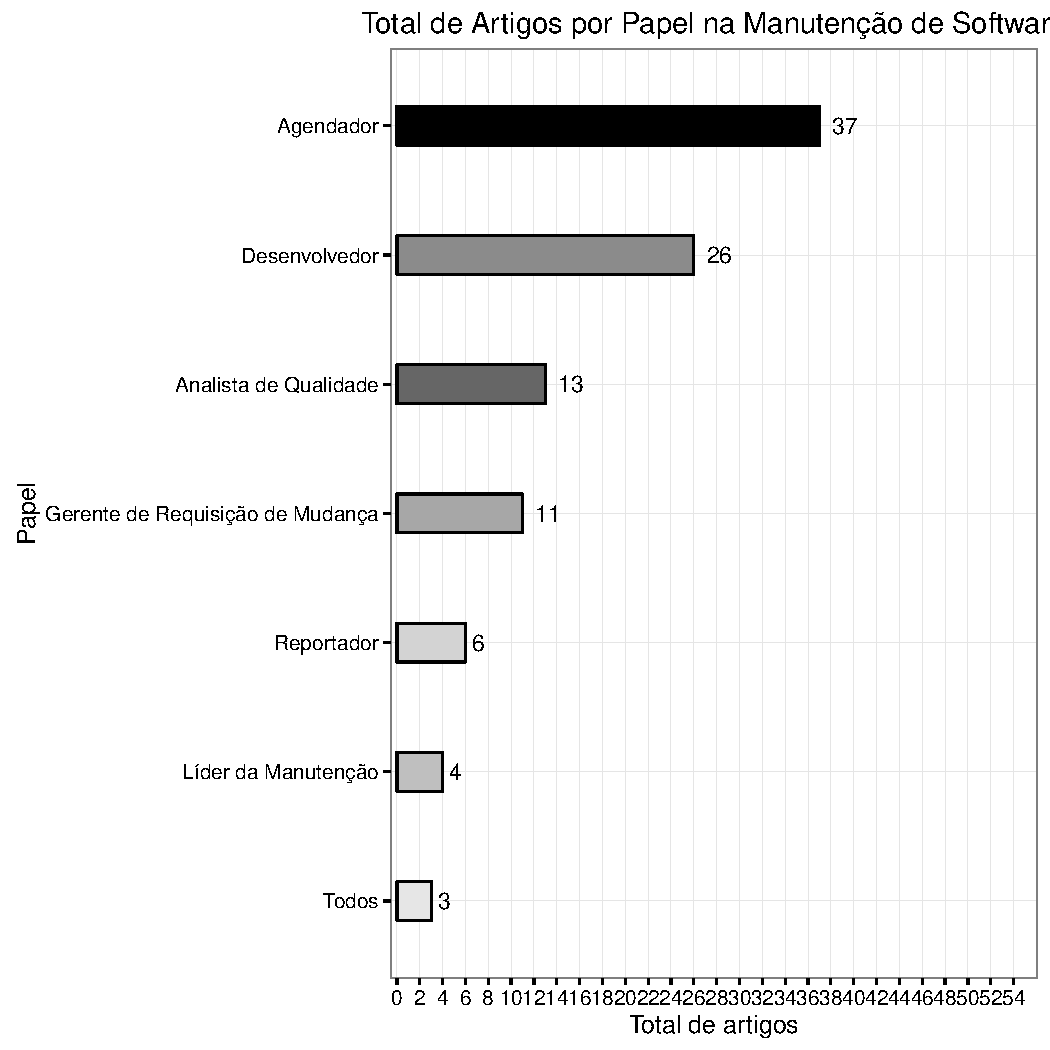
\includegraphics[width=0.8\linewidth]{chapter-mapeamento-sistematico/img/grafico_papel_por_artigo.pdf}
	\caption{Total de artigos por papel na manutenção de
		software}\label{fig:graf_papel_por_artigo} \end{figure}

\paragraph{Agendador} Esta função têm como principal objetivo atribuição das
RM’s para o desenvolvedor mais apto~\cite{banitaan2013decoba}. O processo de
atribuição de RM's deve ser realizado de acordo com a carga de trabalho do
desenvolvedor e com a prioridade que foi atribuída à
RM~\cite{chawla2015automated}.

Neste contexto, os estudos têm focado em apresentar soluções de atribuição
automática~\cite{banitaan2013decoba, shokripour2012automatic, somasundaram2012automatic, Naguib2013, Zhang2014, Zanetti2013};
classificação automatizada~\cite{gegick2010identifying,liu2014faceted, behl2014bug, chawla2015automated,tian2015automated}; visualização da fila de
RM's~\cite{izquierdo2015gila}; agrupamento (clusters) das
requisições~\cite{liu2014faceted}; identificação do tempo necessário à conclusão
da RM (time to fix)~\cite{hosseini2012market,
	Bhattacharya:2011:BTP:1985441.1985472}; sumarização das informações contidas
na RM~\cite{mani2012ausum}; determinação de RM'S duplicadas~\cite{Sun2011,
	Wu2011a}.

Apesar da lista de artigos apresentada em cada tópico não ser exaustiva, os
resultados demonstram um foco maior no suporte à atribuição e categorização das
RM's apresentando soluções automatizadas para estas atividades.

%Existe possivelmente uma crença que é possível melhorar a produtividade do
%processo de manutenção de software reduzindo o esforço de encontrar o
%desenvolvedor mais apto.

\paragraph{Desenvolvedor} Ao Desenvolvedor cabe aplicar as ações que irão
produzir o resultado solicitado/esperado na RM\@. Os estudos nesta categoria
deveriam suportar atividades tais como codificação, depuração e testes. No
suporte ao desenvolvedor identificamos estudos que propõem à atribuição de RM's
a um conjunto de desenvolvedores, em contraposição da tradicional atribuição ao
único programador~\cite{banitaan2013decoba}, visando  minimizar os pro\-ble\-mas
decorrentes da propriedade de código e propiciar um maior nivelamento de
informações entre os membros da equipe. Não obstante, o maior grupo de estudos
nesta categoria está relacionada à ajuda ao desenvolvedor de vincular um
determinado problema do software à sua efetiva origem, ou seja, ao código
fonte~\cite{corley2011recovering,Wong:2014:BBF:2705615.2706096,
	Thung:2014:BIT:2635868.2661678,Nguyen:2012:MAR:2393596.2393671,thung2013automatic,
	Romo:2015:TAT:2745802.2745833}. Nesta mesma categoria verificamos estudos
que dão suporte ao desenvolvedor em classificar à RM que lhe foi atribuída, em
especial aquelas que estão relacionadas às questões de segurança do
sistema~\cite{gegick2010identifying} ou aquelas RM's que possam impedir a
resolução de outras
(blocking-bugs)~\cite{ValdiviaGarcia:2014:CPB:2597073.2597099}

\paragraph{Analista de Qualidade} Cabe ao Analista de qualidade avaliar se uma
RM foi solucionada por um Desenvolvedor afim de verificar se a RM foi
corretamente resolvida. Neste sentido, melhorias em FGRM's que visam facilitar
as atividades deste papel podem estar relacionadas ao processo de teste de
software.

De maneira similar ao que ocorre na classe do Desenvolvedor verificamos uma
prevalência dos estudos visam determinar uma ligação entre um problema de
software e o código
fonte~\cite{corley2011recovering,Wong:2014:BBF:2705615.2706096,
	Thung:2014:BIT:2635868.2661678,Nguyen:2012:MAR:2393596.2393671,thung2013automatic,
	Romo:2015:TAT:2745802.2745833}. Verificamos ainda estudos que tentam
predizer a probabilidade que determinada RM será
reaberta~\cite{xia2015automatic}, o que pode ajudar ao Analista de Qualidade na
priorização das requisições com alta possibilidade de reabertura

\paragraph{Gerente de Requisição de	Mudança} O papel que representa esta classe
está vinculado à gestão do processo de manutenção de software, em especial por
decidir se uma RM será aceita ou rejeitada. Neste contexto, melhorias
relacionadas à classificação quanto ao nível de
segurança~\cite{gegick2010identifying, zhang2011bug, ValdiviaGarcia:2014:CPB:2597073.2597099}, identificação de
duplicações~\cite{hindle2016contextual, sun2010discriminative, alipour2013contextual, banerjee2012automated}.

O estudos que fazem parte desta classe destacam que um considerável conhecimento
sobre o projeto é necessário bem como  a capacidade de negociação com os
desenvolvedores e demais partes interessadas são importantes para desempenho de
papel. Todavia, tendo em vista o esforço e tempo gasto por esta tarefa,
especialmente quando realizada manualmente, seria importante que as FGRM's
automatizassem algumas destas atividades.

\paragraph{Reportador} Conforme discutido anteriormente os dados contidos nas
RM'S são fundamentais em diversas abordagens de melhorias das funcionalidades
das FGRM\@. Esta relevância ainda é maior nos estudos que fazem uso de técnicas
de Recuperação da Informação. As FGRM deveria dar suporte ao Reportador que, na
maioria, é o primeiro a registrar as informações que serão necessárias à solução
da RM\@.

Muitos dos estudos que fazem parte desta categoria  partem da premissa que
melhorar a qualidade dos dados na RM é o ponto de partida para tratar outros
problemas relacionados ao processo de manutenção de
software~\cite{moran2015auto, Moran:2015:EAA:2786805.2807557, Bettenburg2008a}.
Neste sentido verificamos estudos para autocompletar as informações fornecidas
pelo Reportador~\cite{moran2015auto}, suporte a reprodução do
problema~\cite{Moran:2015:EAA:2786805.2807557}; análise da qualidade da
informação fornecida~\cite{Bettenburg2008a, Tu:2014:MQI:2677832.2677844}. Esta
categoria também contempla um estudo que visa detectar se o problema relatado
por uma RM corresponde ao problema relatado por outra que já foi
registrada~\cite{Thung2014}.

\paragraph{Chefe da Manutenção} De forma similar ao Gerente de Requisição de
Mudança as melhorias de funcionalidades proposta nesta categoria estão
vinculadas à gestão de manter software. Conforme o esquema de  classificação de
papeis utilizado neste estudo, o Chefe da Manutenção têm por responsabilidade
definir os padrões e procedimentos que compõe o processo de manutenção que será
utilizado. Para ajudar nesta tarefa alguns estudo  vêm propondo melhorar a
alocação de Tarefas do processo de resolução das Requisições de
Mudanças~\cite{netto2010automated}. Outros estudos visam mensurar o esforço
necessário para solucionar determinada RM~\cite{Vijayakumar2014, Nagwani2010}, o
que podem ajudar ao Chefe no planejamento de liberações de novas versões do
sistema que está sendo mantido.

\paragraph{Todos} Esta categoria abarca os estudos para o qual a melhoria
proposta possui impacto positivo para todos os papéis envolvidos na manutenção
de software. A definição que o foco da melhoria é geral decorre do que foi dito
como objetivos dos autores dos estudos que fazem parte desta categoria ou ainda
por não ser possível determinar uma atividade específica sendo beneficiada.

Conforme pode ser observado, os estudos estão relacionados principalmente com a
melhoria da  visualização das informações contidas nas RM's~\cite{hora2012bug,
	takama2013application, dal2014bug}. Os aperfeiçoamentos podem estar
vinculadas a questões de usabilidade das ferramentas, como por exemplo a
navegabilidade entre as RM's~\cite{dal2014bug}.

\subsection{Ferramentas Estendidas}
\label{sub:ferrramentas_extendidas}

Conforme verificamos nas seções anteriores diversos estudos vêm sendo propostos
na li\-te\-ra\-tu\-ra com o objetivo de melhorar as atividades relacionadas à
manutenção de software. Não observamos em nossos estudos que grande parte das
melhorias propostas não foram implementadas em alguma FGRM de forma a permitir
avaliações pelos profissionais envolvidos em manutenção de software. Do total de
64 estudos que foram utilizados neste mapeamento apenas 4 fazem parte das
funcionalidade de uma FGRM\@.

%\begin{figure}[htpb] \centering
	%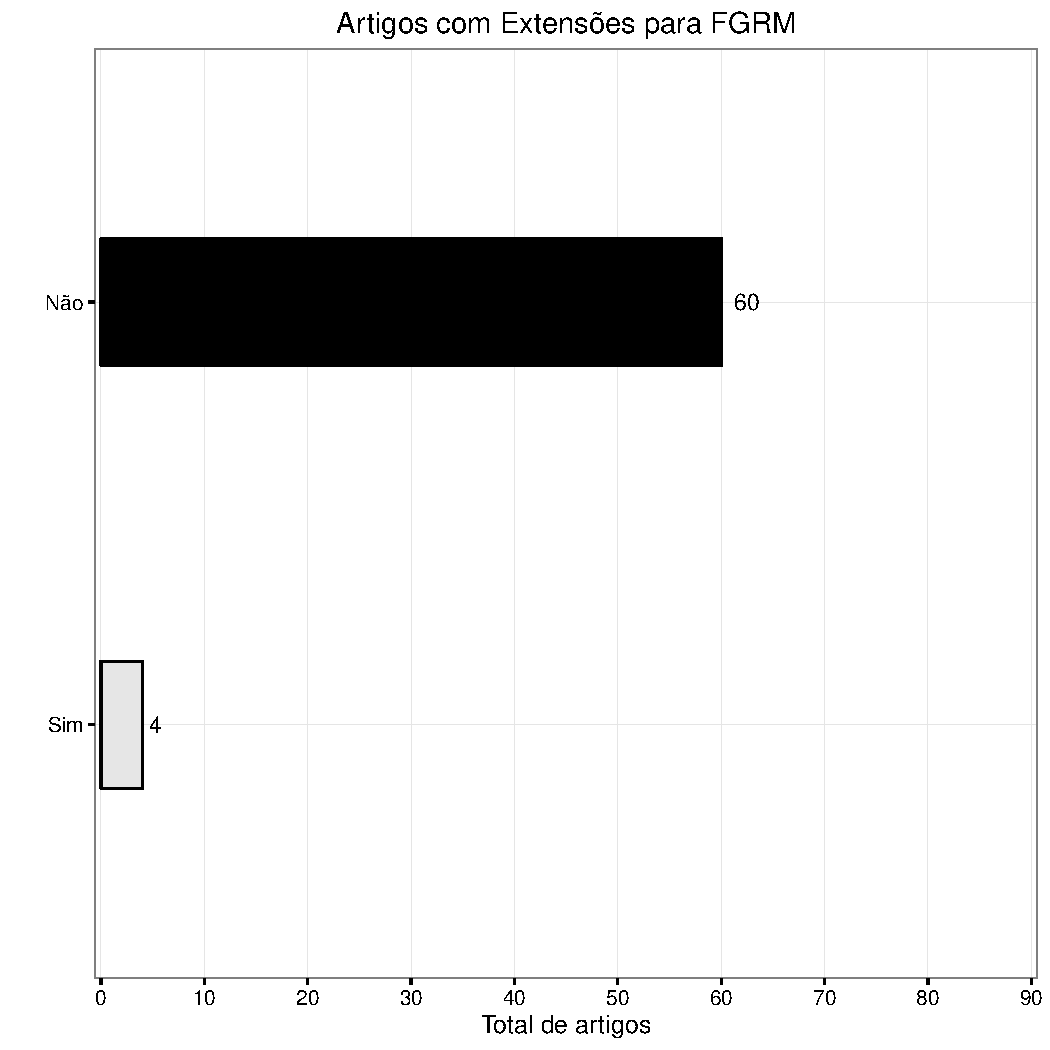
\includegraphics[width=0.8\linewidth]{chapter-mapeamento-sistematico/img/grafico_virou_extensao.pdf}
	%\caption{Total de estudos que são extensões para FGRM}
	%\label{fig:grafico_virou_extensao}
%\end{figure}

Cabe ressaltar que no escopo de determinado estudo pode não esta prevista a
efetiva transformação da melhoria proposta de modo a ser utilizada efetivamente
pelo seu público-alvo, como por exemplo, a criação ou melhoria de uma
funcionalidade de determinada FGRM\@. Ademais, não está no escopo deste estudo
avaliar ou discutir a facilidade que as FGRM possuem para criar novas
funcionalidades ou melhorias. 

%Contudo, o nosso entendimento é que como um maior número de melhorias proposta
%na literatura sendo utilizadas pelos profissionais envolvidos em manutenção de
%software poderia melhorar a qualidade das soluções propostas mediante a redução
%da diferença entre o estado-da-prática com o estado-da-arte. 

%\section{Discussão} \label{sec:discussao}


\section{Limitações e Ameaças à Validade} 
\label{sec:map_limitacoes_ameacas}

Alguns dos procedimentos adotados neste trabalho não acompanharam exatamente as
diretrizes existente na literatura para condução de uma Mapeamento Sistemático.
Um único investigador selecionou os estudos candidatos e este mesmo revisor teve
a responsabilidade de analisar o artigos que seriam incluídos ou excluídos.

O mapeamento realizado neste estudo utilizou o método de aplicação de sentenças
de busca nas bases de dados selecionadas para coletar os estudos primários.
Outros estudos utilizam além da estratégia descrita fazem de uma técnica
conhecida  como ``bola de neve" (snowballing)~\cite{wohlin2014guidelines} onde
as referências dos estudos primários podem ser usadas para o compor o conjunto
de artigos do mapeamento. Neste sentido, ao usarmos uma única estratégia podemos
ter perdido estudos relevantes e, portanto, subestimar a extensão dos resultados
encontrados. Em particular, por termos optado por escolher artigos apenas em
língua inglesa também pode ter havido falta de material publicado em revistas e
conferências nacionais. Assim, nossos resultados devem ser considerados apenas
com base em artigos em inglês contidos nas bases de dados escolhidas  e em
especial publicados nas principais conferências da área de Engenharia de
Software.

O fato de um único pesquisador ter sido o responsável pela análise dos estudos
pode significar que alguns dos dados coletados podem ser errôneas. O processo de
seleção e validação dos estudos primários pode levar a problemas de extração e
agregação das informações quando há um grande número de artigos ou os dados são
complexos~\cite{keele2007guidelines}. No entanto, neste estudo secundário, houve
poucos estudos primários e os dados extraídos eram relativamente objetivos.
Desta forma, não esperamos erros de extração. Cabe ressaltar que apesar do
processo de validação ter sido executado por um único pesquisador, os critérios
de qualidade foram avaliados independentemente por dois pesquisadores, desta
forma minimizando a inclusão de estudos cuja qualidade comprometa os resultados.

No tocante as questões deste estudo  é  possível que as perguntas de pesquisa
definidas possam não abranger completamente o campo de investigação sobre as
funcionalidades das FGRM's. No entanto, algumas discussões com membros do
projeto e especialistas em Manutenção de Software foram realizadas para validar
as perguntas. Assim, mesmo que não tenhamos considerado o melhor conjunto de
questões, tentamos abordar as indagações mais frequentes e abertas no campo,
tanto do ponto de vista do praticante como do investigador.

Como as bases de dados digitais não funcionam com regras de pesquisa compatíveis
entre si, todas as sequências de pesquisa foram adaptadas e calibradas para cada
banco de dados digital. No entanto, não conhecemos todas as regras que as bases
de dados digitais utilizam para procurar um documento. Neste sentido, a forma
que as sentenças de busca foram estruturadas podem não ser a mais otimizada para
seleção do maior número de estudos relevantes para o estudo.

\section{Trabalhos Relacionados}
\label{sec:map_trabalhos_relacionados}

No estudo proposto por Kagdi e outros~\cite{kagdi2012assigning} foi realizada
uma revisão da literatura sobre abordagens para mineração de repositórios de
relatos de problema de software. No contexto daquele trabalho este tipo de
repositório pode ser comparado à uma FGRM\@. O resultado foi uma taxonomia
baseada em quatro classes: o tipo de repositório extraído (o que), o propósito
(por que), o método proposto (como) e o método de avaliação (qualidade). No
entanto, sua taxonomia não fornece um entendimento extensivo sobre as
investigações em repositórios de RM. De acordo com seus critérios de exclusão
para estudos, eles estavam muito preocupados com estudos que abordavam mudanças
evolutivas de artefatos de software investigando múltiplos repositórios de
software. Como consequência, muitos estudos que usaram dados de um repositório
único estavam além de seu escopo.

Por outro lado, o estudo realizado neste trabalho aumentou o escopo das
funcionalidades oferecidas pelas FGRM possibilitando uma visão mais abrangente
do estado da arte deste tipo de estudo. Uma outra diferença com o trabalho de
Kagdi ~\cite{kagdi2012assigning} é que sua taxonomia considera as técnicas e
métodos para mineração de repositórios de software como o foco principal do seu
estudo, por lado este trabalho considera as FGRM, sobre o prisma de suas
funcionalidades, como entidades de primeira classe.

No estudo realizado por Cavalcanti e outros~\cite{cavalcanti2014challenges}
houve a classificação de estudos sobre repositórios de RM em desafios e
oportunidades.  Desafios referem-se a problemas enfrentados na gestão das RM's,
enquanto oportunidades referem-se às vantagens proporcionadas pelos dados
obtidos das  RM's para o desenvolvimento de software. Além disso os autores
utilizam a taxonomia proposta por Canfora e Cerulo\cite{cerulo2004taxonomy}. O
esquema de classificação consiste em duas visões sobrepostas: uma taxonomia
vertical que classifica os modelos de Recuperação da Informação (Information
Retrieve - IR) com relação ao seu conjunto de características básicas; e uma
taxonomia horizontal que classifica os objetos de IR com respeito as suas
tarefas, forma e contexto.

Nosso trabalho estende a classificação realizada por Cavalcanti tendo em vista
que avalia as funcionalidades das FGRM's  que encaixam no conceito de
repositórios de RM's. Contudo, o nosso foco está em como as funcionalidades
daquele tipo de ferramenta vêm sendo melhoradas em contrapartida do outro estudo
que visa mapear os desafios e oportunidades de pesquisa na área.

%\section{Resumo do Capítulo} \label{sec:resumo_capitulo}